\documentclass[10pt, a4paper]{amsart}

\usepackage[ngerman,english]{babel}

\usepackage[latin1]{inputenc}
\usepackage{graphicx}
\usepackage{subfigure}
\usepackage{xcolor}
\usepackage{cite}
\usepackage{babelbib}
\usepackage{multicol}
\usepackage{bbm}
\usepackage{arabtex}
\usepackage{booktabs}
\usepackage[T1]{fontenc}



\usepackage[all]{xy}
\usepackage{amsmath}
\usepackage{amsfonts}
\usepackage{amssymb}
\usepackage[colorlinks, linkcolor=red]{hyperref}  
\title{About the joint measurability of observables}
\author{Alejandro Agust\'i Mart\'{i}nez-Soria  Gallo}
%Margins
%\topmargin -1.0 in
%\textheight 23 cm
%\textwidth 14.0cm
%\oddsidemargin -.5cm
%\evensidemargin -.5cm



% % % ANGLAIS
\newtheorem{theorem}{Theorem}[section]
\newtheorem{lemma}{Lemma}[section]
\newtheorem{proposition}{Proposition}[section]
\newtheorem{example}{Example}[section]
\newtheorem{definition}{Definition}[section]
\newtheorem{corollary}{Corollary}[section]
\newtheorem{hype}{Hypothesis}[section]
\newtheorem{remark}{Remark}[section]


\newcommand{\seethis}{\textcolor{red}{$ \mathbb{SEE} $}\ }
\newcommand{\continue}[1][!]{\textcolor{red}{\emph{Continue #1}}}
\newcommand{\comment}[1]{\marginpar{{\color{red}\tiny #1}}}
\newcommand{\ket}[1]{\left| #1\right\rangle}
\newcommand{\bra}[1]{\left\langle #1\right|}
\newcommand{\projector}[1]{\ket{#1}\!\!\bra{#1}}
\newcommand{\braket}[2]{\left \langle #1 \right|\left.\! #2\right\rangle}
\newcommand{\tr}{\mathrm{tr}}



\newcommand{\bbone}{\ensuremath{\resizebox{5pt}{5.8pt}{1}\hspace{-3.5pt}1}}
\newcommand{\N}{\mathcal{N}}

\newcommand{\defeq}{\overset{\mathrm{def}}{=}}

\usepackage{setspace}
\setstretch{1.5}



\begin{document}
\nocite{*}
%\tableofcontents

\begin{center}
\hrulefill
\end{center}
\vspace{1cm}
\maketitle
\begin{center}
\hrulefill
\end{center}
\begin{center}
\vspace{1cm}
\begin{minipage}{.7\textwidth}
\centering
\textit{Mem\`{o}ria presentada per a l'obtenci\'{o} dels t\'{i}tols de graduat en f\'{i}sica i graduat en matem\`{a}tiques.}
\end{minipage}
\end{center}
\vspace{3cm}
\begin{center}
 \textit{Dirigit per:}\\
\begin{tabular}{ll}
\sc Prof. Dr. Ram\'{o}n Mu\~{n}oz Tapia & \sc Prof. Dr. Andreas Winter\\
\multicolumn{2}{c}{Grup d'informaci\'{o} qu\`{a}ntica}\\
\multicolumn{2}{c}{Universitat aut\`{o}noma de Barcelona}
\end{tabular}
\end{center}
\vfill
\begin{center}
Bellaterra, 4 de setembre del 2014
\end{center}
\thispagestyle{empty}

\newpage
\setcounter{page}{0} 

\thispagestyle{empty}
\tableofcontents

\newpage
\thispagestyle{empty}
\setcounter{page}{0} 
\ 
\vspace{6cm}
\begin{flushright}
\scalebox{1}{\<laulaahu, laulaa Alssa-----rAbu, lam---------------A waa.sila Alssayra ba.hi------------_taN `ani Alm------------------------------------------------------------A'$ \ldots $>}\\
\<ma.h-----mowd darwy^s>\\
\end{flushright}
\begin{flushleft}
\textit{Were it not for it, were it not for the mirage, [he] would not continue the journey in search for water\ldots}\\
Mahmoud darwish
\end{flushleft}
\newpage

 
%\tableofcontents
%\newpage

\section{Introduction}
This report deals with some aspects about the joint measurability of quantum observables. Since W. Heisenberg reviewed the concepts of momentum and position, it has been known that Quantum Mechanics furnishes the impossibility of measuring them together, i.e., it is not possible to measure the one without disturbing the other. This fact holds for many other sets of observables, and it is commonly known by the name of \textit{complementarity}. \\
Some of the examples taught regularly in introductory Quantum Mechanics courses also deal with these constraints in the quantum measurement, however they are rarely presented in its most generality. The mathematical model describing observables in these courses has severe limitations concerning both theoretical and experimental aspects. Even at the beginning of Quantum Mechanics there were doubts whether or not 
when  measuring  the position of some quantum particle the outcome or probability distribution was really that of the model, or otherwise some other \textit{fuzzy} version of it. It is looking for a complete \textit{Theory of Measurement} that many aspects discussed in this report arose for the first time. One of these new properties in the Theory of Measurement is the concept of noise, which we will see plays an important r\^{o}le in questions of measurement. \\
In this project we have put our focus on two outcome observables, i.e., physical measurable properties that may have as an outcome one given value or another. We have developed geometrical methods (\textit{joint measurability graphs}) to visualize and characterize the joint measurability of any set of two outcome observables, together with constraints for noise which must be added to the system in order to make them jointly measurable. \\
 In section $2$ we will define exactly what we understand by a \textit{general} observable. We have devoted section $3$ to introduce shortly the mathematical idea of joint measurability. Section $4$ constitutes the \textit{corpus} of the project. There we discuss in full length properties for two outcome observables based on the work in \cite{wolfgarcia}. We have corrected a claim appearing in \cite{wolfgarcia} and we have provided refinements and possible solutions to issues caused by problems arising from the mistake. 
\newpage
\section{Positive operator valued measures} % (fold)
\label{sec:introduction}


% section introduction (end)

\subsection{Projective measurements}
\label{subsection:projection_measurements}

It has been pointed out that the best way to describe the measurement process in the quantum theory is by considering a class of positive operators. Let us illustrate some features as a way of introduction. \\

Let $\mathcal{H} $ be a $n$-dimensional Hilbert space. Suppose we have a physical observable represented by an hermitian operator $A$\footnote{For simplicity's sake we do not differentiate between an observable or physical property and its assigned operator.}. Suppose that the operator is discrete,  finite and is not degenerated. Then we can find a spectral decomposition given by 

\begin{equation}\label{eq:finite_sharp_observable_selfadjoint}
A = \sum_{i=1}^{n} \alpha _{i}\projector{\alpha _{i}}, 
\end{equation}  

where $\{\ket{\alpha_1},\ldots, \ket{\alpha_n} \}$ is an orthonormal basis of $\mathcal{H}$.
The outcome space of a measurement of observable $A$ is given by the set $\Omega = \{\alpha_1, \ldots , \alpha_n\}$, this is, these are the values that one can measure considering the observable $A$. The axioms of quantum mechanics say that if a measure appartus happens to measure $\alpha_i$ on a state $\ket{\psi}$, then the state immediately after the measurement is $\ket{\alpha_i}$. It is also stated that the probability of measuring $\alpha_i$ on a state $\ket{\psi}$ is 
$$
p(\alpha_{i}) =
|\braket{\alpha_i}{\psi}|^2 = \braket{\psi}{\alpha_i}\braket{\alpha_i}{\psi}
=
\tr \left\{ \projector{\alpha_i}\projector{\psi} \right\}.
$$
If we use the formulation considering statistical mixtures then we would have a trace one positive operator $\rho \in \mathcal{L}(\mathcal{H})$ as the state of the system and the probability of measuring $\alpha_{i}$ would then be 
\[
p(\alpha_{i}) =
\tr \left \{ 
\projector{\alpha_{i}} \rho
\right \}.
\]
Analogously, the probability of measuring $\alpha_{i}$ or $\alpha_{j}$, i.e., the probability that the measurement lies within the set $\{\alpha_{i}, \alpha_{j}\}$, provided that $i\neq j$ is 
\[
p(\{\alpha_{i}, \alpha_{j}\})=
\tr\left \{
\left (
\projector{\alpha_{i}}+\projector{\alpha_{j}}
\right )\rho
\right \}
=
p(\alpha_{i})
+
p(\alpha_{j}).
\]

By considering these last equations, one can see that in fact we have defined a probability measure 
on $2^{\Omega}$, this being the set of the parts of $\Omega$. Therefore, for every element $X$ of $2^{\Omega}$ we can assign the probability $p(X)$ as before. \\

Altogether we actually see  that as far as the measurement is concerned, given a Hilbert space $\mathcal{H}$, all the information of the observable's measurement is encoded in the outcome space $\Omega$ and the set of operators $\left \{\projector{\alpha_{i}}\mid i\in \{1,\ldots , n\}\right \}$.
So the observable is an association of a subset of $\Omega$ (or an element of $2^{\Omega}$) with some operators acting on $\mathcal{H}$, which in this case it would translate into
\[
\{\alpha_{i_{1}}, \ldots, \alpha_{i_{r}}\}\longmapsto \projector{\alpha_{i_{1}}}+\cdots + \projector{\alpha_{i_{r}}}.
\]
It is also worth noticing that for the measurement of probabilities only a certain kind of operators are needed. Indeed operators needn't be projectors but just positive, so that the expected value is always positive and it makes sense to extract from every operator a probability value. 



\subsection{POVM}
We will define what we understand by an \textit{observable} following the footsteps and hints of section \ref{subsection:projection_measurements}.
So let $\mathcal{H}$ be a Hilbert space and let $\rho \in \mathcal{L}(\mathcal{H})$ be a state, i.e., a linear operator acting on $\mathcal{H}$ having trace one. From now on, $\Omega$ will be an outcome space associated with an observable and $\mathcal{F}$ the possible combinations of elements of this $\Omega$ we can calculate probabilities of, i.e., $\mathcal{F}$ is a $\sigma$-Algebra attached to $\Omega$. 


\begin{definition}
\label{def:operator_valued_measure}
Let $(\Omega, \mathcal{F})$ be as above. A map $\mathsf{A}: \mathcal{F}\to \mathcal{L}(\mathcal{H})$ is an \textit{operator valued measure} if and only if the following statements are true:
    \begin{enumerate}
        \item $\mathsf{A}(\emptyset) = 0 $.
        \item Let $\{X_{i}\mid i\in \mathbb{N}\}$ be a countable subset of $\mathcal{F}$. If $X_{i}\cap X_{j} = \emptyset$ for $i\neq j$ and $i,j\in\mathbb{N}$ then 
        \[
 \tr\left \{ 
 \mathsf{A}\left (
 \bigcup_{i\in\mathbb{N}} X_{i}
 \right )
  \rho
 \right \}
 =
  \sum_{i\in\mathbb{N}}\tr\left \{
\mathsf{A}(X_{i})\rho  
  \right \}        . 
        \]
    \end{enumerate}
\end{definition}

Note that for the case that the dimension of the Hilbert space is $1$, the above definition is just the definition of a measure. 

\begin{definition}
Inside the framework of definition \ref{def:operator_valued_measure}:
\begin{enumerate}
\item an operator valued measure $\mathsf{A}:\mathcal{F}\to \mathcal{L}(\mathcal{H})$
is called an \emph{observable} if and only if $\mathsf{A}(X)$ is positive semi-definite for all $X\in \mathcal{F}$ and $\mathsf{A}(\Omega) = 1$. We refer to them also as \textit{positive operator valued measure} or in short POVM. 
\item an observable is called \emph{sharp} if and only if $\mathsf{A}(X)$ is a projector for every $X\in \mathcal{F}$, i.e., $\mathsf{A}(X)^{2}=\mathsf{A}(X)$.  
\end{enumerate} 
\end{definition}
These last definitions are quite general, maybe even they are too general for the purposes of this report, however in proposition \ref{proposition:universality_of_noise_general} we make use of this general framework to prove a proposition. Let show this definition in the simple case of a discrete and finite outcome space $\Omega$. In this case $\Omega = \{\alpha_{1}, \ldots , \alpha_{n}\}$ and since the nature of $\alpha_{k}$ is not important for the purpose of measuring, we may as well call $\alpha_{k}$ simply $k$, so that $\Omega = \{1, \ldots , n\}$. In this case we have for every element of $\Omega$ a positive operator $A_{i}\defeq \mathsf{A}(i) $. So we have a set of positive operators $\{A_{i}, i\in \{1, \ldots , n\}\}$ which fulfill the condition 
$$
\sum_{i}A_{i} = 1
$$
for being $\mathsf{A}$ and observable. In the case of a sharp observable, every $A_{i}$ is of the form $\projector{i}$ for some $\ket{i}\in \mathcal{H}$.   \\

%\begin{example}\label{example:Selfadjoint_operators_are_sharp}
Sharp observables of course are meant to be the self-adjoint operators representing observables that are commonly introduced in 
Quantum Mechanics courses. Returning to the example of last section with the operator $A$ in equation \ref{eq:finite_sharp_observable_selfadjoint}, we made the case that for every possible outcome $\alpha_{j}$ we had the projector $\projector{\alpha_{j}}$ that would give us the propability of measuring $\alpha_{j}$ in the sate $\ket{\phi}$ by $\tr \{\projector{\alpha_{j}}\projector{\phi}\}$. Theoretically this class of observables has a very important property, which has to do with the name \textit{sharp}. Let us suppose we are measuring $A$ on a system which is in the state $\ket{\phi} = \ket{\alpha_{j}}$, since $A$ is sharp, it is composed from projectors and we suppose that all projectors are orthogonal, then we have the following condition on the probability of $\ket{\phi}$
\begin{equation}\label{eq:sharp_observables_property}
\forall i  \quad \tr\{ A(\alpha_{i}) \projector{\phi}\} = \delta_{ij}. 
\end{equation}

In this case, for this particular state $\ket{\phi}$ the distribution is as sharp as a distribution can get. In general sharp observables can get 
arbitrarily sharp, like the position observable, where we can perform experiments to lessen the uncertainty $\sigma_{x}$.  \\

However imagine we do not know the start state $\ket{\phi}$ or this state is in a statistical mixture $\rho$ such that $\rho^{2}\neq \rho$, i.e., such that $\rho \neq \projector{\psi}$ for any $\ket{\psi}$. In this case it is not anymore possible to find a $\rho$ such that $\rho^{2}\neq \rho$
having the property of equation \ref{eq:sharp_observables_property}. \\

In this way POVM's act as real measurements \cite{ludwig1953messprozess} since they do not have the \textit{sharpness} property. 
Of course if we consider Quantum mechanics to be a complete theory of measurement, taking into consideration the dimension $d$ of the Hilber Space $\mathcal{H}$, if we were to content ourselves with \textit{sharp} observables we would not be able to consider  measurements with more than $d$ outcomes, which in the framework of experimentation would be a dramatic hindrance. \\

POVM's give therefore the idea that we should be able to consider any probabilistic-valid distribution we want. They are indeed objects that 
cater an infinity of probability distributions by definition. This means, more concretely, if $(\mathsf{A},\Omega_{A}, \mathcal{F}_{A})$ is a POVM, that for every $\rho$ we get a probability distribution over $\mathcal{F}_{A}$. Indeed, we consider the function that to every $U\in \mathcal{F}_{A}$ assigns the number $\tr \{A(U) \rho\}$. This function is by definition of $A$ a probability distribution over $\mathcal{F}_{A}$. 
 

\subsection{Neumark's theorem}


POVM arise naturally from bipartite systems. In essence, the measurement process is a coupling between the system to be measured $A$ and the system measuring $B$ \cite{ludwig1953messprozess}.
The reading process takes place in $B$, and it is an irreversible process.  This means conceptually that reading the information in $B$ after the coupling may cease to be a \textit{sharp} reading, i.e., when one looks at the probability distribution of the readings in $B$, the structure 
does not comply with the one of a sharp observable.\\

However, there is a way around, which is known as \textit{Neumark's theorem } at it is stated below \cite{beneduci2014joint}.
\begin{theorem}
Let $A$ be a POVM over a given Hilbert space $\mathcal{H}$. Then there exists a sharp observable $A^{+}$ on an extended Hilbert space $\mathcal{H}^{+}$ such that if $P:\mathcal{H}^{+}\to \mathcal{H}$ is the projection from the extended Hilbert space to the former then for every $\ket{\psi}\in \mathcal{H}$ 
$$
A\ket{\psi}  = 
P A^{+}\ket{\psi}.
$$
\end{theorem} 
In simple words what the theorem states is that every POVM can actually be thought as a sharp observable on a bigger Hilbert space. 
Therefore the nature of POVM's gets clarified by it, since any POVM is either sharp or is a partial trace of a \textit{bigger} sharp observable. 





\newpage
\section{Join-mesurability of POVM's} % (fold)
\label{sec:join_mesurability_of_povm}


\subsection{Definition and properties}

\begin{definition}[joint measurability]\label{definition:Join_measurability}
Let $\{\mathsf{A}_{i}\mid i\in \N  = \{1, \ldots , n\}\}$ be a set of POVM's with outcome spaces $\Omega_{A_{i}}$ and $\sigma$-algebras $\mathcal{F}_{A_{i}}$. We say that they are jointly measurable if there exists a POVM $R$ with outcome space $ \Omega_{A_{1}}\times \cdots \times \Omega_{A_{n}}$ and $\sigma$-algebra $\mathcal{F}_{A_{1}}\otimes \cdots \otimes \mathcal{F}_{A_{n}}$ such that every $ \mathsf{A}_{i}$ is a marginal of $R$, i.e., for every $i\in \N$ and every $U\in \mathcal{F}_{A_{i}}$
$$
\mathsf{A}_{i}(U) = Z(\Omega_{A_{1}}\times \cdots \Omega_{A_{i-1}}\times U \times \Omega_{A_{i+1}} \times \cdots \times \Omega_{A_{n}} ) 
$$ 

\end{definition}

Let us illustrate this somewhat general definition with an example of sharp observables. Suppose therefore that 
$$
\hat{A} = \sum_{i} \alpha_{i} \projector{\alpha_{i}}, \qquad \hat{B} = \sum_{i}\beta_{j}\projector{\beta_{i}}
$$
are two self-adjoint operators. To build the POVM's out of the two self-adjoint operators we  consider the outcome spaces $\Omega_{A} = \{\alpha_{i}\}$ and $\Omega_{B} = \{\beta_{i}\}$ and secondly we consider the map 
$$\mathsf{A}:
\{\alpha_{i_{1}}, \ldots , \alpha_{i_{n}}\}\mapsto \projector{\alpha_{i_{1}}} + \cdots + \projector{\alpha_{i_{n}}}.
$$
 Let us call this map $\mathsf{A}$ (resp. $\mathsf{B}$). As it is known from Quantum Mechanics, $\hat{A}$ and $\hat{B}$ are called jointly measurable if and only if they commute since only then we can find a common eigenbasis for both operators. Therefore we could find vectors $\ket{\alpha_{i} \beta_{j}}$ such that $\hat{A}\ket{\alpha_{i} \beta_{j}} = \alpha_{i}\ket{\alpha_{i}\beta_{j}}$ and  $\hat{B}\ket{\alpha_{i} \beta_{j}} = \beta_{j}\ket{\alpha_{i}\beta_{j}}$, which it is interpreted as that the state $\ket{\alpha_{i}\beta_{j}}$ has both the property $\alpha_{i}$ and $\beta_{j}$ \textit{at the same time}.In this sense, only considering commutativity  it is meaningful to consider both properties at the same time.\\

Consider now a pure state $\ket{\psi} $, the probability of measuring $\alpha_{i}$ is of course given by $|\braket{\alpha_{i}}{\psi}|^{2} = \tr\{\projector{\alpha_{i}}\projector{\psi}\}$ and after having measured $\alpha_{i}$, the state $\psi$ collapses irreversibly to $\alpha_{i}$. If we perform another measurement $B$ and we measure $\beta_{j}$, the probability for it is $\tr\{\projector{\alpha_{i}}\projector{\beta_{j}} \}$.\\

If we consider therefore the POVM $Z = A\cdot B$ having as outcome space $\Omega_{A}\times\Omega_{B}$ and as $\sigma$-algebra $\mathcal{F}_{A}\otimes \mathcal{F}_{B}$, it fulfills the following relations:
$$
A(\alpha_{i} ) = Z(\alpha_{i}, \Omega_{B}) = \sum_{\beta \in \Omega_{B}}Z(\alpha_{i}, \beta), \quad B(\beta_{j})=Z(\Omega_{A},\beta) = \sum_{\alpha \in \Omega_{A}} Z(\alpha, \beta_{j})
$$
so we could think that we have found the joint measure for $A$ and $B$. But, notice that we have not used anywhere the fact that $\hat{A}$ and $\hat{B}$ are commute. So we could be falsely led to think that everything is jointly measurable! However, that is not the case. In general nothing ensures the semidefinite positivity of 
$$
Z(\alpha, \beta ) = \projector{\alpha} \projector{\beta}
$$
even though both $\projector{\alpha}$ and $\projector{\beta}$ are positive. It is a theorem of the functional analysis \cite{lysternik1968elemente} that the product of positive operators is ensured to be positive only if they commute. Therefore $Z$ would be a joint measure if all projectors commute which implies the commutation of $\hat{A}$ and $\hat{B}$. 





\subsection{Adding noise}
\label{subsec:Adding_noise}
Given two non-jointly measurable  POVM's $\mathsf{A}$ and $\mathsf{B}$, it is possible to make them joint measurable by \textit{adding} noise into them? What do we understand by noise?  Let us illustrate what is meant by it through an example. Suppose the outcome space of $\mathsf{A}$ is $\{a_{1}, \ldots , a_{n}\}$ and suppose we perform an experiment to measure $\mathsf{A}$ several times, say $M$ times where $M$ should be big enough. Suppose the measurement gets each time states $\rho$ which are assumed to be equally prepared. Then considering the relative frequencies of every $a_{i}\in \Omega_{A}$, i.e. the times we have measured $a_{i}$ divided by $M$, if $M$ is big enough we could identify this relative frequency $f(a_{i})$ with the probability, i.e., 
$$
f(a_{i}) \approx \tr \{\rho \mathsf{A}(a_{i})\}
$$
and we could have a graph such as in figure \ref{fig:pure_vs_noise} in blue.

\begin{figure}[h]
\centering
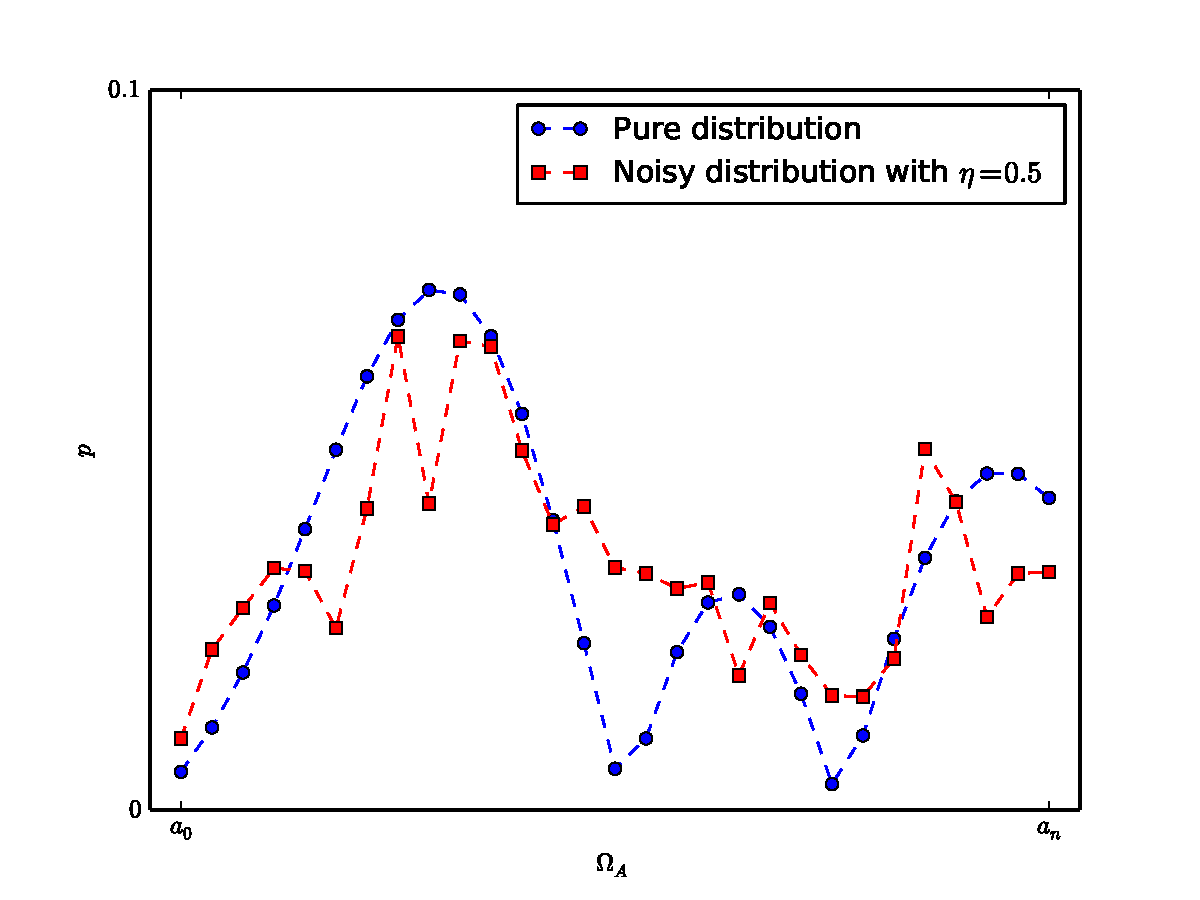
\includegraphics[scale=.6]{images/pure_vs_noise.pdf}
\caption{Graphical representation of the distribution of a given observable $\mathsf{A}$ (in blue) compared with some noisy distribution of the same $\mathsf{A}$(in red). The lines have been added to give also a feeling of how a noisy distribution in the case of a continuous observable would look like. }
\label{fig:pure_vs_noise}
\end{figure}


In practice however we never get such a distribution, or we are not sure to have the real distribution, so one says that there is noise in the system. 
The measuring process is a macroscopic process between some quantum system and a bigger one, where a thermodynamic irreversible process takes action (see \cite{LudwigQuantenmechanik} or \cite{ludwig1953messprozess}). In this process many effects may take place leading to mistakes in the reading of some sensor. These factors are noise sources, and we can mathematically model this influence by taking a convex combination of POVM's, in the case of $\mathsf{A}$ for example we could take another POVM $E$ having too as outcome space $\Omega_{A}$ and representing the noise. A convex combination is provided taking a parameter $\eta\in [0,1]$ and considering the new POVM 
$$
\mathsf{A}_{\eta} = (1-\eta)\mathsf{A} + \eta E.
$$
In figure \ref{fig:pure_vs_noise} we can see a representation of how some results would look like if we were to note down the results of the measurements on some random state $\rho $ and if we could compare the noisy distribution with the pure one. We see that as an overall effect what this tells us is that we actually make gradually less sharp the information until all the information that is left is the unusable information from $E$, which again might be a random noise $POVM$. Therefore it is not strange to assume that considering some $\eta $ we could make $\mathsf{A}_{\eta}$ and $\mathsf{B}_{\eta} $ joint measurable, since we lose more and more information as $\eta $ increases. Let us stress that such convex combinations are not a full description of the noise, but a model. For example note that we can never attain from a positive operator $\mathsf{A}(a_{i})$ to make it zero using such a combination, since $\mathsf{A}_{\eta}(a_{i})> 0$ if $\mathsf{A}(a_{i})> 0. $\\













\newpage
\section{Joint measurablility of two-outcome observables}
\label{section:Compatibility of effects}
\paragraph{\bf Nomenclature:} Throughout this section we will call  two outcome observables \textit{effects} interchangeably, although in the literature we find different uses for the word effect. Also, given a positive operator $P$, we may refer to it as an observable, meaning the two outcome observable $\mathsf{P} = \{P , \bbone - P\}$, it is assumed that $P\leq \bbone$. Both $P$ and $\bbone - P$ are called \textit{ POVM elements}, since they conform together the two outcome POVM or observable $\mathsf{P}$.   We will normally note the outcome space of two outcome observables as $\Omega = \{+,-\}$, so that for example $\mathsf{P}(+) = P$ and $\mathsf{P}(-) = \bbone -P$, or otherwise. The association of $+$ to $P$ or $\bbone - P$ is but a matter of preference and language, the physical significance is encoded in $\mathsf{P}$. 
\subsection{Introduction}
\label{subsec::Comp_introdcution}
Some conditions for the joint measurability of effects have already been found in the literature in the form of inequalities of a certain 
set of operators (see \cite{wolfgarcia}).  In what follows we will attempt to present a generalization and correction of some aspects of these results.  \\

The description of the process needs of an explanation of the framework. In the case of $n=2$, one can find quite straightforward methods to check and find conditions for their joint measurability. Let $\{P, \bbone-P\}, \{Q,\bbone-Q\}$ be two observables having both the outcome space $\Omega_{P,Q} = \{+,-\}$. If they are jointly measurable, a set of operators exists $R(i,j)$, $i,j\in\{+,-\}$, for which the coarse-graining condition is satisfied, i.e.
$$
P = R(+,+) + R(+,-), \qquad Q = R(+,+) + R(-,+)
$$ 
$$
\bbone - P = R(-,+) + R(-,-), \qquad \bbone - Q = R(-,+) + R(-,-)
$$ 
The condition proven in \cite{wolfgarcia} states that $P$ and $Q$ are jointly measurable if and only if there exists a positive operator $S$ such that the following requirements are satisfied, 
\begin{equation}\label{eq:two_effects_conditions}
P+Q- \bbone \leq S , \qquad  S \leq P,Q.
\end{equation}
It is a matter of calculation to check the necessity of the condition, simply take \emph{an operator of the $R$-representation which is common to both $P$ and $Q$}, and this will do the trick (i.e., take $R(+,+)$). The sufficiency condition hides some interesting steps; given such an $S$, the conditions $S\leq P,Q$ allow us to define $R(+,-) \defeq P-S$ and $R(-,+) \defeq Q-S$, which by hypothesis are positive. The condition on the left allows us to define both $R(-,-)\defeq\bbone-P-Q+S \geq 0$ (which will be positive) and to establish the validity of the partition of unity condition of $R$, i.e., $1 = \sum_{i,j} R(i,j)$ where $i,j\in \{-,+\}$. Therefore by calling $S = R(+,+)$ we encounter the desired joint-measure. \\

In \cite{wolfgarcia}, the general conditions for $n$ two outcome observables are written down in terms of the joint measure $R$ directly. However it is of our opinion that to research some properties of $n$ observables, this method is quite opaque in the reading. We have developed a general method using a generalization of the operator $S$ rather than $R$ directly. However, as dimension increases the number of $S$'s increases as well and the huge number of inequalities ceases to have the helpful factor it had in the latter simpler case. It is therefore difficult to see properties or possible solutions to problems arising from the joint measurability through the pure inequality framework. Therefore, we have thought of these inequalities as conforming a directed graph with several floors or levels, and we have derived some general properties of these graphs relevant to physical problems. The direction of the graph is intended to give us some hint about the underlying inequalities.     \\ 

We will discuss the structure of the graph defined for the case of $n= 2$ later on, when we prove the equivalence theorem in the following sections (theorem \ref{Theorem:EQUIVALENCE}). There we prove that the considerations above for two observables and for $n$ observables in \cite{wolfgarcia} are equivalent to considering the graph schema: 
\begin{figure}[h]
$$
\xymatrix@ C = 3mm{
\mathbf{0}&&\bbone\ar[dl]\ar[dr]&\\
\mathbf{1}&P\ar[dr]&&Q\ar[dl]\\
\mathbf{2}&&S(1,2) = S\ar[d]&\\
&&0
}
$$
\caption{Directed graph for two effects.}
\label{Fig:2Effects_Intro}
\end{figure}


The fact that for higher dimension (i.e., more than two effects) we do not only have an operator $S$ to determine, makes complicated to \textit{parametrize} these operators. We have to be able to write them in an operational and ordered way  so that we can identify exactly each operator and we can eventually write algorithms to solve the problems. We use a subset approach to the problem, i.e., every operator and the inequalities are defined in terms of subset properties as it will be seen in definition \ref{definition_JMG}, where we define formally the properties of the graphs and we call them \textit{joint measurability} graphs for the sake of readability of the report. 




\newpage

\subsection{Definition of the graph}
 From now on let us define  $\mathcal{N} = \{1, \ldots , n\}$. 

%\input{images/general_graph.tex}

\begin{definition}[Joint measurability graph]\label{definition_JMG}
Let $G = (V,A)$ be a directed graph. The graph $G$ is called a joint measurability graph of dimension $n$ iff the following conditions are met:
\begin{enumerate}
\item $V$ is a set of operators acting on a Hilbert space. 
\item If $(S_{1},S_{2})\in A$ then $S_{1}\geq S_{2}$.
\item  There exists a bijection 
$$
S:2^{\{1,\ldots , n\}}\to V
$$
\item The bijection defines the elements in $A$, 
$$
A = \{
(S(\Omega_{1}), S(\Omega_{2}))\mid
\Omega_{1} \subset \Omega_{2} \mbox{ and } |\Omega_{2}\backslash \Omega_{1}| = 1
\}
$$
%\item $V$ is a subset of linear operators acting on some Hilbert space. 
\item For every $\Omega$,  $\Omega \subseteq \N $ the following defining inequality is satisfied:
\begin{equation}\label{eq:graph_definition_inequality}
R(\Omega)\defeq\sum_{A\subseteq \N\backslash \Omega}  (-1)^{|A|}S(\Omega \cup A)\geq 0
\end{equation}


\end{enumerate}

\end{definition}

Please note that point $2$ is a consequence of point $5$ although this can not be seen easily directly. However it is desirable to include point $2$ in the definition to make it more transparent and readable. Equation \ref{eq:graph_definition_inequality} may seem a little bit difficult to read at first. Despite this fact, it will become clear as we show  the necessity of such a graph in theorem \ref{Theorem:EQUIVALENCE}. For now let us write an example with dimension $3$. In this case we have $\N = \{1,2,3\}$ and $2^{\N} = \{\emptyset ,\{1\},\{2\},\{3\},\{1,2\},\{1,3\},\{2,3\},\{1,2,3\}  \}$.  We write for simplicity $S(1,3)$ instead of $S(\{1,3\})$. Let us write equation \ref{eq:graph_definition_inequality} for $\Omega = \{1,2,3\}$, since in this case $\Omega = \N$ the only possible $A\subset \N\backslash \Omega$ will be $A = \emptyset$, so in this case it reads:
$$
R(\N)  \defeq (-1)^{0}S(\N\cup \emptyset ) = S(\N) \geq 0. 
$$
For $\Omega = \{1,3\}$ for example, $\N\backslash \Omega = \{2\}$, so $A$ can be $\emptyset$ and $\{1\}$, let us write it:
$$
R(1,3) = (-1)^{0}S(\{1,3\}\cup \emptyset ) + (-1)^{1}S(\{1,3\}\cup \{2\}) = S(1,3) - S(\N) \geq 0
$$
and of course the same is valid for $\{1,2\}$ and $\{2,3\}$. From here we get therefore that $S(A_{2}) \geq S(1,2,3) \geq 0$ where of course $A_{2}$ is a subset of $\N$ of cardinality two. Now suppose $\Omega = \{1\}$, then $A$ can be $\{2\}$, $\{3\}$, $\{2,3\}$ or $\emptyset$, equation \ref{eq:graph_definition_inequality} turns therefore into 
$$
S(1) - S(1,3) - S(1,2) + S(\N ) \geq 0
$$
where we can write the same (but slightly different) for $S(2)$ and $S(3)$. Finally for $\Omega = \emptyset$ we can write
$$
S(\emptyset ) - \sum_{i=1}^{3}S(i) + S(1,2)+ S(1,3) + S(2,3) - S(1,2,3) \geq 0.
$$
All these inequalities can be represented in form of a graph. In figure \ref{fig:graph_n_3} we can see the representation of such a directed graph. \\

\begin{figure}[h]
$$
\xymatrix@C=2mm{
\mathbf{0}&&&&S(\emptyset) \ar[dl]\ar[dr]\ar[d]&&&\\
\mathbf{1}&&&S(1)\ar@{-->}[dr]\ar[d]&S(2)\ar[dl]\ar[dr]&S(3)\ar[d]\ar@{-->}[dl]&&\\
\mathbf{2}&&&S(1,2)\ar[dr]&S(1,3)\ar@{-->}[d]&S(2,3)\ar[dl]&&\\
\mathbf{3}&&&&S(1,2,3)\ar[d]&&&\\
&&&&0&&&\\
}
$$
\caption{Joint measurability graph for $n=3$.}
\label{fig:graph_n_3}
\end{figure}
We can find a thumb-rule to find the inequalities without having to look at the subsets (compare also with section \ref{subsec::Comp_introdcution}). Just take any element $S(\Omega)$ and look at the storey it is in, i.e., $\mathbf{0}, \mathbf{1}, \mathbf{2}$ or $\mathbf{3}$. Then substract everything connected to $S(\Omega)$  lying in the storey immediately beneath, then add everything connected to the elements substracted of the next storey to them, etc\ldots Let us illustrate through an example; take for instance $S(2)$ which is in the storey $\mathbf{1}$ (because $\{2\}$ has one element), connected to it beneath are $S(1,2)$ and $S(2,3)$, so we have to substract them, i.e., $S(2) - S(1,2)-S(2,3)$. We are not yet quiet there, we have to add the element connected to $S(1,2)$ and $S(2,3)$, which is only $S(1,2,3) = S(\N)$. Furthermore being a joint measurability means that the result must be greater or equal zero, so 
$$
S(2) - S(1,2)-S(2,3) + S(1,2,3) \geq 0.
$$

%From now on we will denote by $(V, A)$ a fixed $n$-dimensional joint measurability graph and $S$ a fixed associated defining map.

For the following considerations the following lemma will prove to be useful. 

\begin{lemma}\label{lemma:ROMEGA_AND_SOMEGA}
Let $\N = \{1, \ldots , n\}$ and $\Omega \subseteq \N $. Let $S,R : 2^{\N}\to \mathcal{R}$ be two functions taking values in any $\mathbb{C}$ ring $\mathcal{R}$. The two functions fulfill the relation
\begin{align}\label{Prop:ROmega_presentation}
R(\Omega)=\sum_{A\subseteq \N\backslash \Omega } (-1)^{|A|}S(\Omega \cup A)
\end{align}
if and only if they also fulfill  

\begin{align}\label{S_Omega_R_representation}
S(\Omega) = 
\sum_{A\subseteq \N\backslash \Omega } R(\Omega\cup A)
\end{align}
which can be understood as a coarse-grain property. 
\end{lemma}

\begin{proof}
We begin by showing that equation \ref{Prop:ROmega_presentation} implies \ref{S_Omega_R_representation}.
Let us denote the right-hand side of equation \ref{S_Omega_R_representation} by $\Gamma$. By definition, every term appearing in the summation of $\Gamma$ is 
$$
R ( \Omega \cup A) =
\sum_{A' \subseteq \N \backslash (\Omega \cup A)}
(-1)^{|A'|}
S(\Omega \cup A \cup A' )
$$
and with it we can write for $\Gamma$
\begin{align*}
\Gamma &= 
\sum_{A\subseteq \N \backslash \Omega}
\sum_{A' \subseteq \N \backslash (\Omega \cup A)}
(-1)^{|A'|}
S(\Omega \cup A \cup A' )\\
&=
\sum_{A' \subseteq \N \backslash \Omega}
(-1)^{|A'|}
S(\Omega \cup A' )
+
\sum_{\substack{A\subseteq \N \backslash \Omega\\ |A|\neq 0} }
\sum_{A' \subseteq \N \backslash (\Omega \cup A)}
(-1)^{|A'|}
S(\Omega \cup A \cup A' )\\
&= 
R(\Omega) 
+
\sum_{\substack{A\subseteq \N \backslash \Omega\\ |A|\neq 0} }
\sum_{A' \subseteq \N \backslash (\Omega \cup A)}
(-1)^{|A'|}
S(\Omega \cup A \cup A' )
\end{align*}

where we have separated the summation by taking $A = \emptyset $ on one and $A \neq \emptyset$ on the other,  we have used the definition of $R(\Omega )$. The second last summation depends therefore on $A$ and $A'$, where $A'$ has in its turn also a dependence on $A$. We will change of variable for the summation by taking 
$$
Z = A \cup A'
$$
and finding a summation over $Z$. Let us note however what are the ranges of $|A|$, $|A'|$ and $|Z|$ all together:
$$
\left .
\begin{matrix}
|A| &\in & \{ 1, \ldots , n -|\Omega | \}\\
|A'| &\in& \{ 0 , \ldots , n-|\Omega| - |A| \}
\end{matrix}
\right \}
\Rightarrow
|Z| \in \{1, \ldots , n-|\Omega| \}
$$ 

From the latter consideration it follows that $Z$ can be any subset of $\N \backslash \Omega$ with cardinality greater or equal than $1$. 
Let us consider a given $Z$, there are several forms of obtaining it from sets $A$ and $A'$. For example if $|A| = 1$, $A'$ is automatically determined by $Z\backslash A$ and there are $\binom{|Z|}{1} $ ways of doing it, which correspond of course to the possible  subsets of $Z$ of length $1$. Writing the possibilities in dependence of the cardinality of $A$ there are therefore
$$
\sum_{i=1}^{|Z|}\binom{|Z|}{i} = 2^{|Z|}-1
$$
possible ways of producing $Z = A \cup A'$, what means that $S(\Omega \cup Z)$ appears $2^{|Z|}-1$ times in $\Gamma - R(\Omega)$. In order to sum up all these terms we have to consider the change of sign according to the cardinality of $A'$, which is $|Z|-|A|$ or in the sum above $|Z|-i$. We can therefore write 
$$
\sum_{i=1}^{|Z|}(-1)^{|Z|-i}\binom{|Z|}{i}S(\Omega \cup Z) = [(1-1)^{|Z|}-(-1)^{|Z|}]S(\Omega \cup Z)
=
-(-1)^{|Z|}S(\Omega \cup Z)
$$

This means however that we can rewrite $\Gamma$ simply in terms of $Z$ in the following way 
\begin{align*}
\Gamma &= R(\Omega) + 
\sum_{
\substack{Z\subseteq \N\backslash \Omega \\
|Z| \neq 0}}
(-1)(-1)^{|Z|}S(\Omega \cup Z)\\
& = 
R(\Omega) -
\sum_{
\substack{
Z\subseteq \N\backslash \Omega \\
|Z| \neq 0}}
(-1)^{|Z|}S(\Omega \cup Z) = S(\Omega)
\end{align*}
which is the exactly $S(\Omega)$ by definition on equation \ref{eq:graph_definition_inequality}. \\

Implication of equation \ref{Prop:ROmega_presentation} from equation \ref{S_Omega_R_representation} is shown similarly. We denote as before the right-hand side of equation \ref{Prop:ROmega_presentation} as $\Gamma$ and express every term of the sum in function of the assumption:
\begin{align*}
\Gamma &=
 \sum_{A\subseteq \N \backslash \Omega}\sum_{A'\subseteq \N \backslash (\Omega \cup A)}(-1)^{A}  R(\Omega \cup A \cup A')\\
 &= R(\Omega ) + 
 \underset{|A|+|A'|\neq 0}{\sum_{A\subseteq \N \backslash \Omega}\sum_{A'\subseteq \N \backslash (\Omega \cup A)}}
 (-1)^{A}  R(\Omega \cup A \cup A')
\end{align*}
where of course we have put out of the summation the pair $(A, A')$ where both of them where the emptyset. Now the only constraint on the sets $Z = A \cup A'$, $A$ and $A'$ is that $A$ and $A'$ can not be the empty set at the same time. Following the reasoning of before and for given $Z = A \cup A'$ we find that the sum of the elements $R(\Omega \cup Z )$ is 
$$
(-1)^{0}\binom{|Z|}{0} + (-1)^{1}\binom{|Z|}{1} + \ldots + (-1)^{|Z|}\binom{|Z|}{|Z|} = (1-1)^{|Z|} = 0.
$$
As before, writing the equation changing variables with $Z$ we find that $\Gamma = R(\Omega )$ as desired. 

\end{proof}
































\newpage
\subsection{Graph equivalence}
We set out to prove the equivalence of \emph{joint measurability} graphs and joint measurable effects. For that we prove the following main theorem: 
\begin{theorem}\label{Theorem:EQUIVALENCE}
Let
 $\{P_{1}, \ldots , P_{n}\}$ be a set of effects. These effects are jointly-measurable if and only if there exists an $n$-dimensional joint measurability graph $(V, A, S)$ such that $S(i) = P_{i}$ for every $i\in  \{ 1,\ldots , n \}$ and \emph{$S(\emptyset ) = \bbone$}. 
\end{theorem}
\begin{proof}

Let us begin by showing the \textbf{necessity}. Let us suppose the effects take values on $\{+,-\}$, so that $P_{i}$ is the operator related to $+$. If they are joint measurable then there exists a POVM $R: \{+,-\}^{n}\to \mathcal{L}(\mathcal{H})$ fulfilling 
$$
P_{i} = \sum_{\substack{ t_{i} = +\\ t_{k} \in \{+,-\} }} R (t_{1}, \ldots, t_{i}, \ldots , t_{n}) .
$$
For the sake of readability let us denote, $R(t_{1}, \ldots , t_{n} ) $, where  some of the $t_{k}$ are equal to $+$, by this subset of indexes, i.e., we do not write the indexes for which $t_{k} = -$, e.g. :
$$
R(+, - , +, - , \ldots, \overset{k}{+}, - , \ldots , +) =: R(\{1,3,k,n\}) = R(1,3,k,n).
$$ 
Let $\N = \{1, \ldots , n\}$ and $S$ be a function over $2^{\N} $ defined as 
$$
S( \Omega )  = \sum_{A\subset \N\backslash \Omega} R(\Omega \cup A), \quad \forall \Omega \subseteq \N. 
$$
Since $\N $ is finite and $R ( A ) $ is well-defined for every $A \subset \N$, $S$ is well-defined and finite. Let us remark that this is in fact a mere general coarse-graining property since as a consequence of the definition $S(i) = P_{i}$\footnote{For simplicity we write $S(i_{1}, \ldots , i_{t})$ instead of $S(\{i_{1}, \ldots , i_{t}\})$} and $S(\emptyset ) = \bbone$. Consider 
$V = \{ S(\Omega) \mid \Omega \subseteq \N \}$ 
and 
$A = \{ (S(\Omega_{1}), S(\Omega_{2}))\mid \Omega_{1}\subseteq \Omega_{2}, |\Omega_{2}\backslash \Omega_{1}| = 1 \}$, 
we claim that with it $(A,V,S)$ is a joint measurability graph. Since we have defined $A$ and $V$ through $S$ there are only two conditions left to be shown, i.e.:
\begin{itemize}
\item $(S(\Omega_{1} ) , S(\Omega_{2}))\in V  \Rightarrow S(\Omega_{1} ) \geq S(\Omega_{2}) $: This is the case since every term appearing in definition of $S(\Omega_{2} ) $ appears also on the definition of $S(\Omega_{1})$ due to $\Omega_{1} \subseteq \Omega_{2} $. 
\item That 
$$
R(\Omega)=\sum_{A\subseteq \N\backslash \Omega } (-1)^{|A|}S(\Omega \cup A)
$$
is a consequence of lemma \ref{lemma:ROMEGA_AND_SOMEGA}. Moreover, the expression is positive semi-definite for all $\Omega \subseteq \N$ by hypothesis. 
\end{itemize}

Not we proceed to show the \textbf{sufficiency}. Suppose therefore that there exists a joint measurability graph $(V,A,S)$ meeting the requirements 
of the hypothesis. The joint measurablility of the effects follows directly from the definition of the graph. Let us define $R:\{+,-\}^{n}\to \mathcal{L}(\mathcal{H})$ as before, namely from $R(\Omega ) $ of the graph we define $R(+,-,-, \ldots )$ with $+$ in the positions determined by the elements of $\Omega$. They are positive semi-definite and from lemma \ref{lemma:ROMEGA_AND_SOMEGA} we have 
$$
P_{i} = \sum_{A\subset \N\backslash \{i\}}R(\{i\}\cup A) = \sum_{\substack{t_{i} = +\\ t_{k}\in \{+,-\}}}  R(i_{1}, \ldots, t_{i-1},+ , t_{i+1}, \ldots, t_{n})
$$
which gives us the coarse graining condition. The $\sigma$-additivity of $R$ is automatic since $\{+,-\}^{n}$ is finite and $R$ is defined through single elements of the set. 


\end{proof}

We apply the theorem \ref{Theorem:EQUIVALENCE} to the case $n=2$ as an example. Let us therefore consider two jointly measurable effects $\{P_{1}, \bbone - P_{1}\}$ and $\{P_{2}, \bbone - P_{2}\}$. In this case we have the function $S: 2^{\{1,2\}}\to V$ where $S(\emptyset ) = \bbone$ and $S(i) = P_{i}$. We have therefore a $S(1,2)$ such that the following graph is satisfied:
$$
\xymatrix@ C = 3mm{
\mathbf{0}&&\bbone\ar[dl]\ar[dr]&\\
\mathbf{1}&P_{1}\ar[dr]&&P_{2}\ar[dl]\\
\mathbf{2}&&S(1,2) \ar[d]&\\
&&0
}
$$
As expressed in the theorem, if $P_{i}$ is associated with the value $+$ and $\bbone - P_{i}$ with $-$, then for instance $R(1,2)$ means $R(++)$. In this case $0\leq R(++) = S(1,2)$ and 
$$
R(1) = P_{1}- S(1,2) = P_{1}- R(++) = R(+-)\geq 0, \qquad P_{2}- R(++)  = R(-+)\geq 0
$$
and finally 
$$
R(\emptyset) = \bbone - P_{1}-P_{2}+ R(++) = R(--)\geq 0.
$$
These $R(i,j)\geq 0$ form indeed a joint-measure of $P_{1}$ and $P_{2}$, which is exactly the result explained in section \ref{subsec::Comp_introdcution}. In this way, theorem \ref{Theorem:EQUIVALENCE} can be thought of as a generalization of Proposition 1 in \cite{wolfgarcia}. 





\newpage
\subsection{Graphs as semidefinite programs}
\label{subsec:Graphs_as_semidefinite_programs}

As shown in 
\cite{wolfgarcia}
the joint measurablility problem of observables can be cast in the form of a semidefinite program. We show this same process making use of the 
graph structure. This is helpful when there is the need of performing a simulation of the joint measurablility of effects or to specify graphically and 
clearly some properties of these so created semidefinite programs. \\

The primal problem of a \textit{semidefinite program} (SDP) (see \cite{vandenberghe1996semidefinite}) consists in minimizing a linear function of a vector $\vec{x}\in \mathbb{R}^{m}$ subjected to a linear matrix inequality constraint, i.e. 
\begin{equation}\label{eq:SDP:GENERAL_FORMULA:PRIMAL}
\min_{\vec{x}} 
\left \{
c^{T}x
\left| 
F_{0}
+
\sum_{i=1}^{m}
x_{i}F_{i}
\geq 0
\right .
\right \}
\end{equation}

where $F_{i} $ are $n$-dimensional symmetric matrices. The data of the problem is therefore $c\in \mathbb{R}^{m}$ and $\{F_{i}\mid i\in \{0,\ldots, m\}\}\subset M_{n}(\mathbb{R})$. This kind of optimization problems is efficiently solvable using methods like \textit{interior-point methods} which are generally used also for linear programs.\\


Let $\{P_{1}, \ldots, P_{n}\}$ be $n$ effects and $G = (V,A,S) $ a potential joint measurability graph that would be associated to the set of effects if these were jointly measurable. Let $\N = \{1, \ldots , n\}$ and $\{Q_{i}\mid i\in\{ 1, \ldots , d \}\}$ be a hermitian basis for the space where the effects are in. Then for every 
$S(A)$ where $A\subset \N $ and $|A| \geq 2$ we write 
$$
S(A) = \sum_{i=1}^{d}x_{i}^{A}Q_{i}.
$$
In this way we define variables $x_{i}^{A}$ for every $A$ such that $|A|\geq 2$. To refer generally to all of them it is important, specially when programming an algorithm, to define any bijection like
$$
\varphi:\{1, \ldots , 2^{n}-n -1\}\longrightarrow \{A \subset \N\mid |A|\geq 2\}
$$ 
which exists since the cardinality of the set on the right is exactly $2^{n}-n-1$. 
Let us define $\vec{x} = (\vec{x}_{1}, \ldots, \vec{x}_{2^{n}-n-1})$ where every $\vec{x}_{i}$ is associated by the bijection $\varphi $ to an element $\varphi(i) = A$ such that 
$$
\vec{x}_{i} = (x_{1}^{\varphi(i) }, \ldots , x_{m}^{\varphi(i) }). 
$$ 
For every element $S(\Omega)$ with $|\Omega| \geq 2$ we write the graph condition as 
$$
\sum_{A\subseteq \N \backslash \Omega} (-1)^{|A|}S(\Omega \cup A)
=
\sum_{A\subseteq \N \backslash \Omega}
\sum_{i = 1}^{d}
x^{\Omega \cup A}_{i}
 (-1)^{|A|}
Q_{i}
\geq 0 
$$
If $\Omega = \{k\}$ then we may write 
$$
P_{k} + 
\sum_{A\subseteq \N \backslash \{k\}}
\sum_{i = 1}^{d}
x^{\{k\} \cup A}_{i}
 (-1)^{|A|}
Q_{i}
\geq 0
$$
and finally if $\Omega = \emptyset$ we change slightly the property of the graph (i.e. $S(\emptyset ) = \bbone$) and set instead $S(\emptyset ) = \lambda \bbone$, where $\lambda \in \mathbb{R}^{+}$, thus 
$$
\lambda\bbone - \sum_{i\in \N} P_{i} +\sum_{\substack{A\subseteq \N\\|A|\geq 2}}
\sum_{i = 1}^{d}
x^{\Omega \cup A}_{i}
 (-1)^{|A|}
Q_{i}
\geq 0.
$$
\begin{figure}[h]
$$
\xymatrix@C=2mm{
&&&\bbone \ar@{-->}[d]_{?}^{?}&&&\\
&&&\lambda\bbone \ar[dl]\ar[dr]\ar[d]&&&\\
&&P_{1}\ar@{-->}[dr]\ar[d]&P_{2}\ar[dl]\ar[dr]&P_{3}\ar[d]\ar@{-->}[dl]&&\\
&&S(1,2)\ar[dr]&S(1,3)\ar@{-->}[d]&S(2,3)\ar[dl]&&\\
&&&S(1,2,3)\ar[d]&&&\\
&&&0&&&
}
$$
\caption{joint measurability graph representation for minimization of SDP-parameter $\lambda$.}
\label{FIG:GRAPHFOR3_SDP}
\end{figure}

These inequalities have the following form 
$$
R(\Omega ) 
=
F_{0}(\Omega) + \sum_{i=0}^{d(2^{n}-n-1)}F_{i}(\Omega)x_{i}\geq 0, \qquad \vec{x} = (x_{0},x_{1}, \ldots , x_{d(2^{n}-n-1)})
$$
which is a constraint of the form of the ones appearing in the definition of semidefinite programs in equation \ref{eq:SDP:GENERAL_FORMULA:PRIMAL} and where we have added to the former vector $\vec{x}$ a real variable $x_{0} = \lambda$ which accounts for the fine-tunning of the parameter $\lambda$. \\

To create a single matrix inequality we can direct sum all terms of the inequalities so as to have 
a large block matrix with all terms of all inequalities. 
$$
F_{i} = \bigoplus_{\Omega \subset \N} F_{i}(\Omega),
$$
and in this way we can write the equivalent inequality 
$$
F_{0} + \sum_{i = 0}^{d(2^{n}-n-1)}x_{i}F_{i}\geq 0
$$
The problem of finding a joint measurability graph, so that the effects will be joint measurable is equivalent to minimizing
$\lambda $ subjected to the constraint above, or subjected to the set of all individual constraints mentioned before In this semidefinite program therefore $c$ will be equal to  $c = (1, 0 , \ldots, 0)\in \mathbb{R}^{d(2^{n}-n-1)+1}$
$$
\min_{\vec{x}} \left \{
c^{T}\vec{x} = \lambda
\left |  
F_{0} + \sum_{i = 0}^{d(2^{n}-n-1)}x_{i}F_{i}\geq 0
\right .
\right \}.
$$
\begin{itemize}
\item If  $\lambda \leq 1$ is the minimum then the effects are joint measurable since the graph can be extended to the unity as shown in figure \ref{FIG:GRAPHFOR3_SDP} with a dashed arrow.   
\item If however $\lambda > 1$ then the  effects $\{P_{i}\}$ are not joint measurable, there exists no joint measure since if it existed we would be able to create a graph such as in figure \ref{FIG:GRAPHFOR3_SDP} with $\lambda = 1$, so at least $\lambda $ should have a value less or equal than $1$.
\textit{It is worth noticing that the set of operators even if $\lambda > 1$ still build a joint measurability graph, with the only change from theorem \ref{Theorem:EQUIVALENCE} consisting in considering $S(\emptyset) = \lambda \mathit{\bbone} $ instead of $\mathit{\bbone} $.  }
\end{itemize}

The last point will be important from now on, so we find convincing building a proposition out of it:
\begin{proposition}\label{proposition:EFFECTS_GRAPHS_JMG}
To every set of two outcome observables $\{P_{1}, \ldots, P_{n}\}$ we can assign a joint measurability graph built up out of the solutions for the SDP composed by them. 
\end{proposition}
Up to now we had seen in theorem \ref{Theorem:EQUIVALENCE} that we could assign JM-graphs to jointly measurable observables, now we can assign them to any set of effects. In principle we could make them joint measurable by adding noise to the system, like for example considering the convex transformation 
$$P_{i}\to (1-\eta) P_{i} +\eta E$$
where $0\leq E\leq \bbone$ is some other effect and $\eta \in [0,1]$ (see section \ref{subsec:Adding_noise}). The problem is of course to know how much noise must be 
added to the system in order to make the effects joint measurable. In other words, we would like to find constraints for $\eta$ such that $\alpha \leq \eta \leq \beta$ for certain $\alpha , \beta \in [0,1]$. These constraints should tell us at least how much noise we have to add and if this amount of noise is enough to ensure the joint measurablility of the observables. \\

In this very sense it has been claimed in \cite{wolfgarcia} that it is possible to define for the case $n = 2$ a distance between the effects accounting for their joint measurablility and amount of noise altogether. Let us therefore consider $\{P_{1}, P_{2}\}$ a set of two effects. If $\lambda(P_{1},P_{2}) \leq 1$ these effects would represent the same point, so the distance will have to be $0$. Consequently, if we want a distance based on the idea of joint measurability, we represent it by 
$$
\mu (\{P_{i}\mid i\in\{ 1,2 \}\}) = 0, \qquad \mbox{whenever } \lambda \leq 1
$$
If however $\lambda >1$ then is this extra amount that could be taken in consideration to find a necessary (and also sufficient) noise constraint. This amount of noise is  $0< \mu = 1-\lambda^{-1} <1$. Therefore the distance the distance in this case is defined to be:
$$
\mu (\{P_{i}\mid i\in \{ 1,2 \}\}) = \max \{0 , 1-\lambda^{-1}\}.
$$
This was claimed however only for the case of two effects. Regrettably, as it turns out, that the above consideration is inconsistent, because it presupposes that $\lambda$ is the same performing the SDP with $\{P_{1},P_{2}\}$, $\{P_{1}, \bbone - P_{2}\}$ etc\ldots For otherwise there can not be a consistent definition of distance.  We we will see that this is the case, $\lambda$ depends on the combination of POVM elements.  We provide later on a correction and a generalization of this fact.  For some coming results the idea of joint measurability \textit{subgraphs} will prove to be useful (e.g. Corollary \ref{corollary:j_wisely_noise_proposition}). We devote next section to their definition and to the prove that they exist. 































\newpage
\subsection{Existence of subgraphs}
In order to use the graph structure to study some aspects about the joint measurability of observables and present them in a graphical and clear way, it has been thought of use to look for substructures in the graph, for example in order  to express the joint measurability of a subset of the effects being studied. For that we see that the joint measurability graphs have associated in a straightforward way smaller structures having the same properties and therefore representing subgraphs. 

\begin{proposition}\label{Propositions:THERE_ARE_SUBGRAPHS}
Let $G = (V,A,S)$ be a $n$-dimensional joint measurability graph and $\N = \{1, \ldots ,n\}$. Then for every $\Omega \subseteq \N $  we can define a \emph{joint measurability subgraph} $\tilde{G} = (\tilde{V}, \tilde{A}, \tilde{S})$ of $G$ in the following way:
\begin{enumerate}
\item ($\tilde{S}: \Omega \to \tilde{V}) = (S\mid_{\N\cap \Omega}: \N\cap \Omega \to V$)
\item $\tilde{A}\subseteq A$
\end{enumerate}

\end{proposition}

\begin{proof}
Let us first check the basic properties. From point one we get that $\tilde{S} = S\mid_{\N \cap \Omega}$ and therefore
$$
\tilde{V} = \{S(A)\mid A \subseteq \Omega\}\subseteq {V}.
$$
which ensures point $1$ in definition \ref{definition_JMG}. 
The second point implies, 
$$
\tilde{A} = \{(S_{1},S_{2}) \mid  ( (S_{1},S_{2})\in A) \wedge ( S_{1},S_{2}\in \tilde{V}) \}.
$$
which implies points $2$ and $4$ in the definition of JM-graph.
If $\tilde{G}$ is to be a joint measurability subgraph then the condition 
$$
\tilde{R}(\tilde{\Omega} ) \defeq
 \sum_{A\subseteq \Omega \backslash \tilde{\Omega}} (-1)^{|A|}\tilde{S}(\tilde{\Omega}\cup A )\geq 0
$$
must be satisfied for every $\tilde{\Omega}\subset \Omega$. This is indeed the case, to prove it let us make use of the fact that $\tilde{V}$ is a subset of ${V}$, then by lemma 
\ref{lemma:ROMEGA_AND_SOMEGA} we know that 
$$
\tilde{S}(\tilde{\Omega}\cup A ) = S(\tilde{\Omega}\cup A ) = \sum_{A'\subseteq N\backslash ( \tilde{\Omega}\cup A ) } R(\tilde{\Omega}\cup A \cup A' ) .
$$
Let us then rewrite the expression for $\tilde{R}(\tilde{\Omega})$ as 
\begin{align*}
\tilde{R}(\tilde{\Omega}) &= 
 \sum_{A\subseteq \Omega \backslash \tilde{\Omega}}
 \sum_{A'\subseteq \N\backslash ( \tilde{\Omega}\cup A ) } 
  (-1)^{|A|}
 R(\tilde{\Omega}\cup A \cup A' )  .
\end{align*}
We need some framework to prove the result. Firstly let us decompose $\N \backslash (\tilde{\Omega}\cup A ) $ into two disjoint sets, 
$$
\N \backslash (\tilde{\Omega}\cup A ) = (\N \backslash \Omega) \cup (\Omega \backslash (\tilde{\Omega }\cup A )  )
$$
so since $A'$ is a subset of the first, we can also decompose $A'$ into two subsets, $A' = I \cup O$, which we think as \emph{inside $\Omega$} and \emph{outside $\Omega$} (compare with figure \ref{fig:subgraph_proof} for clarification). We will study the terms of the sum $\tilde{R}(\tilde{\Omega})$ in function of the cardinality of $A$, where of course $|A|\in \{0 , \ldots , \omega - \tilde{\omega}\}$ where $\tilde{\omega} = |\tilde{\Omega}|$ and $\omega = |\Omega|$. \\
\begin{figure}[h]
\centering
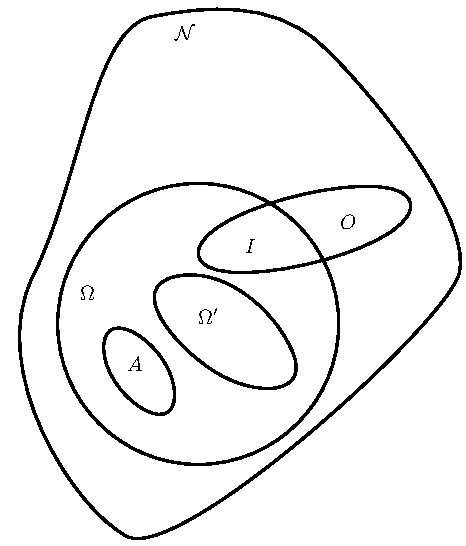
\includegraphics[scale=.7]{images/proof_subgraph.pdf}
\caption{Representation of the sets appearing in the proof of proposition \ref{Propositions:THERE_ARE_SUBGRAPHS}. }
\label{fig:subgraph_proof}
\end{figure}

Let us take a set $A_{k}\subset \Omega \backslash\tilde{\Omega}$ with $|A_{k}| = k$. Then for this set we have in the sum elements of the form 
$$
R ( \tilde{\Omega} \cup A_{k} \cup I_{k} \cup O)
$$
where $ I_{k} \subseteq \Omega\backslash (\tilde{\Omega}\cup A_{k}) $. Consider  terms using $I_{k} = \emptyset$ and let us find  $A\subset \Omega\backslash \tilde{\Omega}$ and $I \subset \Omega \backslash (\tilde{\Omega}\cup A)$ such that 
\begin{equation}\label{Eq:prop:Subgraphs:Equality_of_R_functions}
R ( \tilde{\Omega} \cup A_{k} \cup \emptyset \cup O) = R ( \tilde{\Omega} \cup A \cup I \cup O').
\end{equation}


Note that if this is the case then $\tilde{\Omega} \cup A_{k} \cup \emptyset \cup O =   \tilde{\Omega} \cup A \cup I \cup O' $ and since $O\cap \Omega = \emptyset$ and $ O ' \cap \Omega = \emptyset$ it must follow $A_{k} \cup \emptyset  = A \cup I$ and $O' = O$, where we write everywhere $\emptyset $ to express the lack of the $I$-term in the case of $A_{k}$. If we look for candidates on the level of $A_{k}$ or higher, i.e., we consider $A$ to have $k$ elements or more, the search will fail. Let us suppose that this is indeed the case and there are $(A,I)$ with $|A|\geq k$ such that 
$A\cup I = A_{k}$. This can not be the case since $|A\cup I | = |A| + |I| \geq |A_{k}| = k $, we can only have equality if $|I| = 0$ and $|A| = k$, but then $A = A_{k}$. \\

Let us look now for candidates $(A,I)$ with $|A| = j< k$, in this case the equality \ref{Eq:prop:Subgraphs:Equality_of_R_functions} leads to 
$$
|A| + |I| = |A_{k}| \Rightarrow |I | = k-j.
$$ 
Since $A \cup I = A_{k}$ then $A$ is a subset of $A_{k}$ of $j$ elements, once the subset $A$ is fixed then $I$ is automatically determined via $A_{k}\backslash A $. Therefore there are inside the set of $A$ with $j$ elements exactly $\binom{k}{j}$ possibilities of finding a decomposition like $A\cup I = A_{k}$, moreover the relation 
$$
A_{k}\longleftrightarrow \mathcal{C}_{j}(A_{k})\defeq \{ (A,I) \mid |A|= j, A\cup I = A_{k}  \}
$$
is a bijection. Let us sum now all 
$$(-1)^{|A|}
R(
\tilde{\Omega}
\cup A\cup I \cup O
 ), \qquad (A,I) \in C_{j}(A_{k})
 $$
 where $ j\in \{0, \ldots, k\} $ and $ O \subset \N\backslash \Omega $. Since the $R$-term is the same for all, we will have a coefficient multiplying $R(
\tilde{\Omega}
\cup A\cup I \cup O
 )$, let us call this coefficient $c(A_{k},O)$, this coefficient will be 
 $$
c(A_{k},O ) = (-1)^{k}|C_{k}(A_{k})| + (-1)^{k-1} |C_{k-1}(A_{k})|+ \ldots + (-1)^{0}|C_{0}(A_{k})|
 $$ 
 and since we said that $|C_{j}(A_{k}) | = \binom{k}{j}$ then $c(A_{k},O) = 0$ for $k\geq 1$. \\
 
 The only case where we have $c(A_{k}, O) \neq 0$ is when $k=0$, i.e., $A = \emptyset$, in this case we have 
 $$
\mathcal{C}_{0}(\emptyset) =  \{(\emptyset,\emptyset) \}, \quad c(\emptyset,O ) =1
 $$
 and therefore we have 
 \begin{align*}
 \tilde{R}(\tilde{\Omega})
 &=
 \sum_{k=0}^{\omega - \tilde{\omega}}
 \sum_{\substack{
A\subset \Omega\backslash \tilde{\Omega}\\
|A| = k 
 }}
 \sum_{O\subset \N\backslash \Omega}
 c(A,O)
 R(\tilde{\Omega}\cup A \cup O)
 = 
\sum_{O\subset \N\backslash \Omega}
R(\tilde{\Omega}\cup O)\geq 0
 \end{align*}

\end{proof}
%\begin{figure}[h]
$$
\xymatrix@C=2mm{
&&&\bbone \ar[dl]\ar[dr]\ar@{..>}[d]&&&\\
&&P_{1}\ar@{->}[dr]\ar@{..>}[d]&P_{2}\ar@{..>}[dl]\ar@{..>}[dr]&P_{3}\ar@{..>}[d]\ar@{->}[dl]&&\\
&&S(1,2)\ar@{..>}[dr]&S(1,3)\ar@{..>}[d]&S(2,3)\ar@{..>}[dl]&&\\
&&&\ar[d]S(1,2,3)&&&\\
&&&0&&&
}
$$
\caption{Joint measurability subgraph with $n=3$ and $\Omega = \{1,3\}$.}
\label{fig:subgraphn3omega2}
\end{figure}


Let us illustrate the result with an example. Suppose $\{P_{1}, P_{2}, P_{3}\}$ are joint measurable and let $\N = \{1,2,3\}$. Then by theorem \ref{Theorem:EQUIVALENCE} we can find a joint measurability graph $G = (V,A,S)$ such that figure \ref{fig:subgraphn3omega2} holds. \\
\begin{figure}[h]
$$
\xymatrix@C=2mm{
&&&\bbone \ar[dl]\ar[dr]\ar@{..>}[d]&&&\\
&&P_{1}\ar@{->}[dr]\ar@{..>}[d]&P_{2}\ar@{..>}[dl]\ar@{..>}[dr]&P_{3}\ar@{..>}[d]\ar@{->}[dl]&&\\
&&S(1,2)\ar@{..>}[dr]&S(1,3)\ar@{..>}[d]&S(2,3)\ar@{..>}[dl]&&\\
&&&\ar[d]S(1,2,3)&&&\\
&&&0&&&
}
$$
\caption{Joint measurability subgraph with $n=3$ and $\Omega = \{1,3\}$.}
\label{fig:subgraphn3omega2}
\end{figure}

Suppose now $\Omega = \{1,3\}$ and we want to follow the definition of subgraph to construct it. Following the definition we only need to 
take the effects $P_{1}$ and $P_{3}$ and all the elements they have in common up to $S(A)$ where $|A| = 2$. In figure \ref{fig:subgraphn3omega2} we have drawn too in solid lines the subgraph. By proposition \ref{Propositions:THERE_ARE_SUBGRAPHS} we know that this is a joint measurability subgraph, i.e., we know from the properties of the graph $G$ that 
$\bbone - P_{1}-P_{3} + S(1,3), P_{1}-S(1,3), P_{3}-S(1,3), S(1,3)\geq 0 $. Physically this means two things:
\begin{enumerate}
\item As it is well known any subset of a set of jointly measurable effects is jointly measurable.
\item In the graph $G$ for the joint measurability of the effects we have the joint measurability graph for all combinations of the effects. 
\end{enumerate}
 
 
 
 
 
 
 
 
 
 
 
 
 
 
 
 
 
 
 
 
 
 
 
 
 
\newpage
\subsection{Joint measurability for $n=2$}
\label{subsection:JMforN2}
Consider the two-outcome observables $\{P, \bbone - P\}$ and $\{Q, \bbone - Q\}$, we could build a graph using any combination of elements, $\{P,Q\}$, $\{\bbone - P, Q\}$ etc\ldots Are the parameters coming from the SDP equivalent for every choice of operators? As it may be seen, they are not in general. Take the trivial case where $P =Q = \bbone$ and perform the SDP using $\{\bbone, \bbone\}$ and $\{0,0\}$. Since they are trivially sharp, the joint measure is unique so that we know exactly the $S$ elements we must write on the graphs.  You would have the following representations of the graph:
$$
\xymatrix{
&\alpha\bbone\ar[dl]\ar[dr] &\\
\bbone\ar[dr] && \bbone\ar[dl]\\
&\bbone \ar[d]&\\
&0 &
}
\qquad \qquad
\xymatrix{
&\beta\bbone\ar[dl]\ar[dr] &\\
0\ar[dr] && 0\ar[dl]\\
&0\ar[d]&\\
&0&
}
$$
Of course the infimum value of $\alpha$ so that the graph holds is one and the infimum value of $\beta$ is 0. Despite this fact, notice that both values are less or equal than $1$, which in terms of the information about the joint measurability gives no additional information.
However, as a mathematical problem, this last example hints to the fact that in general an invariance of the SDP parameter depending on the choice of POVM elements is not to be expected. 
We will see through an example that this is indeed too the case for non jointly measurable observables, and we use this fact to discuss a claim provided in \cite{wolfgarcia}, which unfortunately we have found to be false. \\

\paragraph{\bf Claim:}\!\!\cite{wolfgarcia} Let $\{P , \bbone - P\}$ and $\{Q, \bbone - Q\}$ be two observables and let $\lambda_{0}$ be the solution to the SDP constructed by $P$ and $Q$. Then $\eta = \max\{0 , 1-\lambda_{0}^{-1}\}$ is the least number such that 
the two $2$-outcome observables induced by the POVM elements $(1-\eta) P + \eta E$ and $(1-\eta) Q + \eta E$ are jointly measurable \textit{for all} $E$ such that $0\leq E\leq \bbone$. \\

This claim is inconsistent with the fact that there might a dependence of the $\lambda$ SDP parameter on the POVM element choice. Indeed, let us suppose that the parameter $\lambda$ for $(P,Q)$ is different from the parameter $\lambda'$ for $(\bbone - P, \bbone - Q)$.
This means therefore according to the claim that 
$$
(1-\eta)P + \eta E, \qquad
(1-\eta)Q + \eta E, \qquad \forall E( 0\leq E \leq \bbone)
$$
are jointly measurable, exactly like 
$$
(1-\eta')(\bbone -P) + \eta' E', \qquad
(1-\eta')(\bbone -Q) + \eta' E' , \qquad \forall E'( 0\leq E' \leq \bbone)
$$
are. Here $\eta = \max\{0, 1-\lambda^{-1}\}$ and accordingly for $\eta'$. However that the observables directly above are jointly measurable for every choice of $E'$ means that 
$$
(1-\eta')P + \eta' (\bbone - E'), \qquad
(1-\eta')Q + \eta'(\bbone- E') , \qquad \forall E'( 0\leq E' \leq \bbone)
$$
are jointly measurable by definition. Taking $\bbone - E' = E $ we have the same condition as before leading to a contradiction, since by hypothesis   either $\eta < \eta '$ or $\eta' <\eta$. An example of this behavior, and therefore the proof for this fact, is given in the following example:

\subsubsection{Example}
Consider $ P = \alpha \projector{0}$ and $ Q = \bbone - \beta \projector{\phi}$ where $\ket{\phi}$ is such that $\braket{0}{\phi}\neq 0$, $\alpha, \beta \in (0,1)$ and $\ket{\psi} = u \ket{0} + v\ket{1}$. Of course we are considering qubits with basis $\ket{0}$ and $\ket{1}$. 
To consider the reciprocal SDP, i.e., $\tilde{P} = \bbone - \alpha \projector{0}$ and $\tilde{Q} = \beta \projector{\phi}$ notice that the description is exactly the same changing $\alpha \to \beta$ and $\beta \to \alpha$ since $\ket{0} = u\ket{\phi} + \tilde{v}\ket{\phi^{\bot}}$.\\
Let us therefore consider the SDP with $P$ and $Q$. 
From here it is very easy to see which will be the general form of $S$ in the SDP. The condition for $P$ and $S$ is 
$$
P - S \geq 0 \Rightarrow \alpha \projector{0} \geq S
$$
$S$ can not have any projection on $\ket{1}$ since $0 \leq  \bra{1} S \ket{1} \leq \alpha \bra{1}\projector{0}\ket{1} = 0$. 
Since $S$ is a complex positive semidefinite operator, it must be also hermitian. From these two points we deduce that 
$S = t \projector{0}$ where $\alpha - t\geq 0$. 

Since $\ket{\phi} = u \ket{0} + v\ket{1}$ and $Q = \bbone -\beta \projector{\phi}$, we can write $Q$ as 
$$
Q = 
\begin{pmatrix}
1-\beta |u|^{2} & -u v^{*}\\
-u^{*}v & 1 - \beta |v|^{2} 
\end{pmatrix}
$$
For the condition of $Q$ we want 
$$
S \leq Q = \bbone - \beta \projector{\phi} \Rightarrow  t\projector{0} +\beta \projector{\phi} \leq \bbone
$$
so the maximum eigenvalue $\lambda_{q}(t)$ of $t\projector{0} +\beta\projector{\phi}$ can be at most $1$,
$$
\lambda_{q}(t) = \dfrac{\sqrt{(t-\beta)^2  +4 \beta t |u|^2}+t+\beta}{2}\leq 1 . 
$$
Since $\lambda_{q}(t)$ is monotonous increasing, we can find $t_{1}$ such that $\lambda_{q}(t_{1}) = 1$ and then consider the inequality $t\leq t_{1}$. It is a matter of checking that 
$$
t_{1}(\beta) = \dfrac{1-\beta}{1-\beta + \beta |u|^{2}}.
$$
Therefore we have on the one hand $ 0\leq t \leq \alpha$ and on the other $0\leq t\leq t_{1}(\beta)$. 

The SDP parameter inequality, $\lambda \bbone - P - Q + S \geq 0 $ says that 
$$
\lambda \bbone \geq P + Q -S
$$
where $\lambda$ is the infimum of the parameters that fulfill this inequality. Therefore for every $t$, $\lambda$ must be the norm of $P+Q-S$. 
We can write $P+Q-S$ as a matrix,
$$
P + Q - S = 
\begin{pmatrix}
1-\beta |u|^{2} + \alpha - t & -\beta u v^{*}\\
-\beta u^{*}v & 1 - \beta |v|^{2} 
\end{pmatrix}
$$
The maximum eigenvalue of this matrix (the norm) is 
$$
 \lambda(t; \alpha, \beta,u)  = 
\dfrac{\alpha-t+2-\beta
+
\sqrt{
(\beta+ \alpha - t)^{2}
-
4\beta (  \alpha -t  )|u|^2}
}{2}
$$

Therefore this example works by finding an optimal $t$, which must fulfill $t \leq \alpha$ and $t\leq t_1(\beta)$. Of course if $\alpha \leq t_{1}(\beta)$ then the optimal choice for $t$ would be $\alpha$, and otherwise $t_{1}(\beta)$. On $[0,1]$ $t_{1}(x)$ is a monotonous decreasing function, and there is no point $x_{0}\in (0,1)$ for which $t_{1}(x_{0}) = 0$ since $t_{1}(0) = 1$ and $t_{1}(1) = 0$. \\
There exists therefore a point $c\in [0,1]$ for which $c = t_{1}(c)$, this point is given as a function of $u$ by 
$$
c(u) = \dfrac{1}{1+u}.
$$
\begin{figure}[h]
\centering
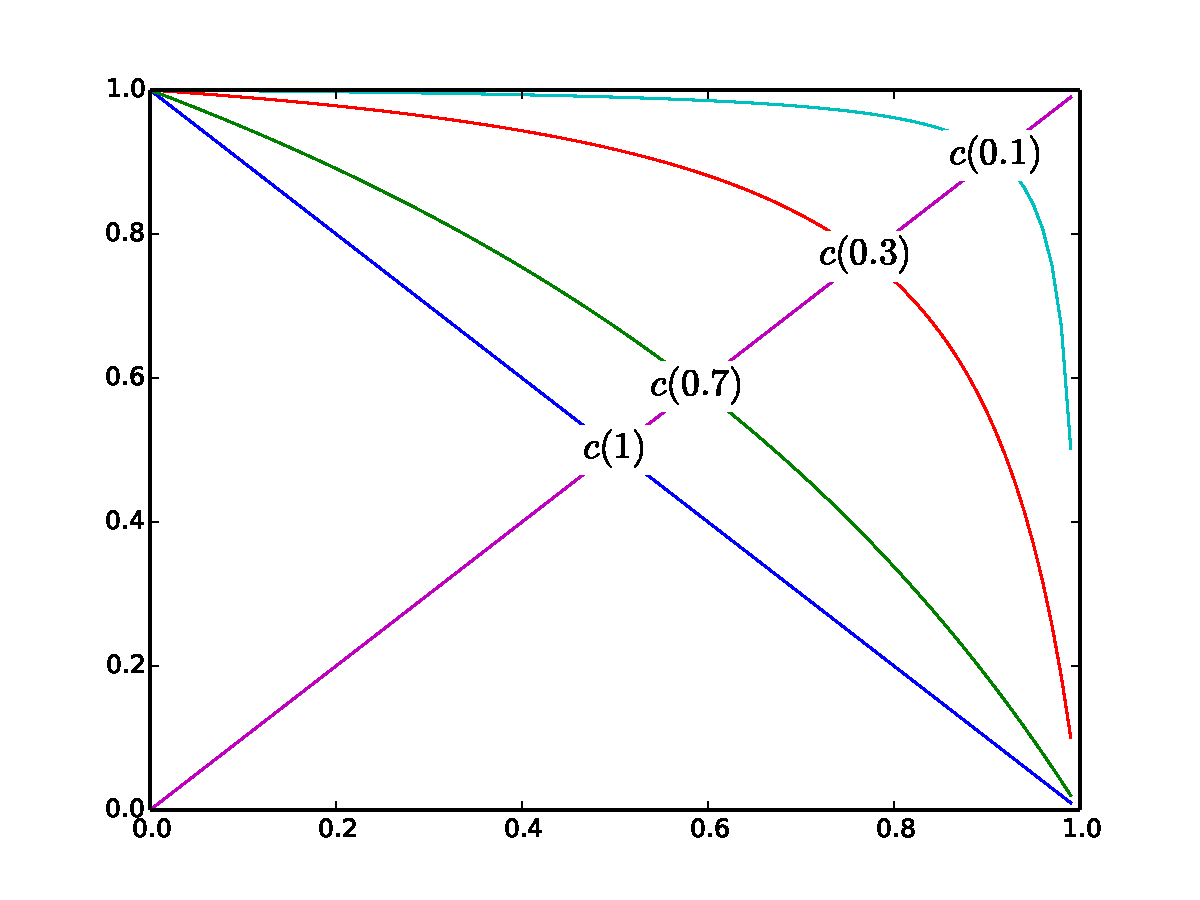
\includegraphics[scale=.6]{images/alpha_t1.pdf}
\caption{Representation of the functions $x\mapsto x$ and $t_{1}(x;u)$ for $u\in\{1,0.7,0.3,0.1\}$. The intersection point $c(u)$ has been drawn too for each $u$.}
\label{fig:alpha_t1}
\end{figure}

Therefore, if $\alpha < c(u)$ we have that $\alpha < t_{1}(x)$ for all $x < c(u)$ (compare with figure \ref{fig:alpha_t1}). This is important since we can choose $\alpha $ and $\beta $ such that $\alpha \leq t_{1}(\beta)$ and $\beta \leq t_{1}(\alpha)$, therefore we would know which is the optimal value of $t$. This is, in the SDP formed by $P$ and $Q$, $t$ would be $\alpha$ since $\alpha \leq t_{1}(\beta)$, we write that as $t_{\alpha\beta} = \alpha$. However, in the SDP formed by $\tilde{P}$ and $\tilde{Q}$, $t$ would be $\beta$ since $\beta \leq t_{1}(\alpha)$, we note it as $t_{\beta\alpha} = \beta$. However, in this cases we have 
$$
\lambda_{\alpha\beta} = \lambda(t_{\alpha\beta};\alpha, \beta, u) =     \dfrac{2-\beta+ \sqrt{\beta^{2}}}{2} = 1,     
$$
and the same for $\lambda_{\beta\alpha}$. Therefore, the set of points 
$$
M_{<<} = \{(\alpha,\beta)\mid \alpha <t_{1}(\beta) , \beta < t_{1}(\beta)\}
$$
lead to a SDP parameter invariant (from $P,Q$ to $\tilde{P}, \tilde{Q}$) and equal to $1$. It is clear that whenever $\alpha = \beta$, the equation for $\lambda(t,\alpha,\beta,u)$ is symmetrical and we have invariance too. There are two sets left to consider, i.e. 
$$
M_{<>}  = \{(\alpha,\beta) \mid \alpha < t_{1}(\beta) , \beta > t_{1}(\alpha), \alpha \neq \beta\}
$$
and 
$$
M_{>>} = \{(\alpha, \beta)\mid \alpha > t_{1}(\beta) , \beta > t_{1}(\alpha),\alpha\neq \beta\}.
$$
For these two sets we make two conjectures. The first is that $M_{<>} = \emptyset$. The second is that the set of points for which $\lambda(t, \alpha, \beta, u)$ is not invariant under the change  $\alpha \leftrightarrow \beta$ is $M_{>>}$. These conjectures are backed by numerical calculations performed using the algorithm found in the appendix \ref{appendix:section:algorithm}. 

\begin{table}[h]
\centering
\caption{Some suitable points where the SDP parameters $\lambda_{\alpha\beta}$ and $\lambda_{\beta\alpha}$ are not equal.}
\label{table:suitable_points}
\begin{tabular}{cccccccc}
\toprule
 $\alpha$ & $\beta$ & $t_{1}(\alpha)$ & $t_{2}(\beta)$ & $u$ &$\lambda_{\alpha\beta}$&$\lambda_{\beta\alpha}$& $\in M_{>>}$? \\
 \midrule
  1.0 & 0.2 & 0.0 & 0.83 & 0.9 & 1.06574 & 1.04497 & yes \\
\hline 0.9 & 0.7 & 0.18 & 0.47 & 0.7 & 1.28205 & 1.33054 & yes \\
\hline 0.8 & 0.9 & 0.28 & 0.15 & 0.8 & 1.3521 & 1.34139 & yes \\
\hline 0.7 & 0.6 & 0.54 & 0.65 & 0.6 & 1.03338 & 1.0372 & yes \\
\hline 0.5 & 0.9 & 0.74 & 0.24 & 0.6 & 1.18529 & 1.11663 & yes \\
\hline 0.4 & 0.9 & 0.86 & 0.31 & 0.5 & 1.07092 & 1.03296 & yes \\
\hline 0.3 & 0.9 & 0.87 & 0.24 & 0.6 & 1.04209 & 1.02238 & yes \\
\hline 0.2 & 0.9 & 0.86 & 0.15 & 0.8 & 1.01945 & 1.01539 & yes \\
\bottomrule
\end{tabular}
\end{table}

Some points where the SDP parameters are not invariant are presented in table \ref{table:suitable_points}. 








\newpage

\subsubsection{Refinement}
A suitable refinement of the \textit{claim} we have found to be the following proposition:

\begin{proposition}\label{proposition:refinement}
   Let $\{P_{1},\mathit{\bbone} - P_{1}\}$  and $\{P_{2}, \mathit{\bbone} - P_{2}\}$ be two observables. 
   Consider the SDP parameter $\lambda_{0} $ coming from considering the SDP for $\{P_{1}, P_{2}\}$. Then the parameter $\eta$ given by  
   $$
\eta  = \max \{0 , 1- \lambda_{0}^{-1}\}   
  $$
is the least number such that $\{(1-\eta) P_{1}, (1-\eta)(\mathit{\bbone} - P_{1}) + \eta \mathit{\bbone}\}$ and $\{(1-\eta) P_{2}, (1-\eta)(\mathit{\bbone} - P_{2}) + \eta \mathit{\bbone}\}$ are jointly measurable. Furthermore, if 
$$
\lambda_{0} \mathit{\bbone} - P _{1} - P_{2} + S_{0} \neq 0
$$ 
where $S_{0}$ is a solution to the SDP, 
there exist some operators $E$ with $0< E< \mathit{\bbone}$ such that the observables 
$\{(1-\eta) P_{i} + \eta E , (1-\eta)P_{i} + \eta (\mathit{\bbone} - E)\}$ are jointly measurables for $i\in\{1,2\}$. 
\end{proposition}
\begin{proof}
Let us suppose that $\lambda_{0} > 1$, for otherwise the claim is automatic since the observables are jointly measurable and $\eta = 0$. The structure of JM-graphs is invariant under multiplication by a positive scalar. Indeed, for every element we have an inequality the sign of which is not changed by the product. Therefore taking $1-\eta = \lambda_{0}^{-1} \in (0,1)$ we have the following representation:
$$
\xymatrix@ C = 2mm{
&\ar[dl]\ar[dr]\lambda_{0} \bbone&\\
P_{1}\ar[dr]&&P_{2}\ar[dl]\\
&S_{0}\ar[d]&\\
&0&
}
\xymatrix{
\\
\ar@{<=>}[rr]^{\times (1-\eta ) }&&\\
\\
}
\xymatrix@ C=-5mm{
&\ar[dl]\ar[dr]\bbone&\\
(1-\eta)P_{1}\ar[dr]&&(1-\eta)P_{2}\ar[dl]\\
&(1-\eta)S_{0}\ar[d]&\\
&0&
}
$$
For the SDP composed by $(1-\eta)P_{1}$ and $(1-\eta)P_{2}$, $1$ is the minimum SDP parameter, since $\lambda_{0}$ was the minimum for $P_{1}$ and $P_{2}$. 
Now consider the SDP for $(1-\eta) P_{i} + \eta E$, 
$$
\begin{matrix}
\bbone - (1-\eta) P_{1} - (1-\eta) P_{2} - 2\eta E + S\geq 0 \\
(1-\eta)P_{i} + \eta E - S \geq 0 \\
S\geq 0
\end{matrix}
$$
If we prove the feasibility of this system for some $S$ and $E$ then they will be jointly measurable. Indeed take $S = (1-\eta) S_{0}$, and $E$ such that 
\begin{equation}\label{eq:refiniement}
\bbone 
\geq\!\!\footnote{
By the properties of $S_{0}$ we know that $-(1-\eta)P_{1} + (1-\eta)S_{0}\leq 0$, so 
$\bbone - (1-\eta)P_{2} - (1-\eta)P_{1} + S \leq \bbone - (1-\eta)P_{2}\leq \bbone$ since $P_{2}\geq 0$. 
}
\bbone - (1-\eta)P_{1} - (1-\eta)P_{2} + (1-\eta) S_{0}
\geq 
2\eta E 
\geq 0
\end{equation}
 If $\lambda_{0}\bbone - P_{1} - P_{2} + S_{0}\neq 0$ equation \ref{eq:refiniement} allow us to find some $0<E<\bbone$ (\textit{near $0$}) such that with this choice of $E$ and $S$ the system's feasibility is fulfilled, i.e.:
$$
\begin{matrix}
\bbone - (1-\eta) P_{1} - (1-\eta) P_{2} - 2\eta E + (1-\eta)S_{0}\geq 0 \\
(1-\eta)P_{i}  - (1-\eta)S_{0} + \eta E\geq  (1-\eta)P_{i}  - (1-\eta)S_{0} \geq 0 \\
S_{0}\geq 0
\end{matrix}
$$
\end{proof}

This proposition is a first step towards a full characterization of the problem. Firstly, the parameter $\eta$ is still dependent on the choice of the POVM elements to build the SDP or the JM-graph with. Therefore, it does not seem to be possible to consider $\eta$ as a \textit{full} descriptor of the noise of the joint measurement of $\{P_{1}, \bbone - P_{1}\}$ and $\{P_{2}, \bbone - P_{2}\}$ as claimed in \cite{wolfgarcia}. We have sought to resolve this problem in proposition \ref{proposition:MUTLIETAN2}, where we have found that such a parameter with the desired interpretation is obtainable. \\
However, before setting out to prove the proposition we may ask about the possibility that depending on the choice of the POVM elements some SDP parameters be less or equal than one and some greater. More explicitly:

\begin{lemma}\label{lemma:invariance_of_lambda_minus_1}
Let $\{P_{1}, P_{2}\}$ and $\{Q_{1}, Q_{2}\}$ bet two. Let $\lambda(i,j)$ be the solution to the SDP problem taking $P_{i}$ and $Q_{j}$.   If there exist $i_{0}, j_{0}\in \{1,2\}$ such that $\lambda ( i_{0}, j_{0})\leq 1 $, then $\lambda ( i,j) \leq 1$ for all $i,j\in\{1,2\}$. 
\end{lemma}
\begin{proof}
Suppose there exist such $(i_{0}, j_{0})$ as in the hypothesis. Then $\{P_{1}, P_{2}\}$ and $\{Q_{1}, Q_{2}\}$ are jointly measurable, which means that we can find a joint measure $R$ and build graphs as in theorem \ref{Theorem:EQUIVALENCE}, which for any choice of $P_{i}$ and $Q_{j}$ would give us a feasibility condition for the SDP parameter $\lambda = 1$, therefore $\lambda (i,j) \leq 1$. 
\end{proof}
 



\begin{proposition}\label{proposition:MUTLIETAN2}
Let $\{P_{1}, P_{2}\}$,  $\{Q_{1}, Q_{2}\}$  and $\lambda(i,j)$ be as in lemma \ref{lemma:invariance_of_lambda_minus_1}. 
\begin{enumerate}
\item    There exists a minimum parameter $\eta \in [0,1]$ such that 
$\{(1-\eta)P_{i}, \mathit{\bbone} - (1-\eta)P_{i}\}$ and $\{(1-\eta)Q_{j}, \mathit{\bbone} - (1-\eta)Q_{j}\}$ are jointly measurable for any choice of $i,j\in \{1,2\}$. This parameter is given by $\max\{0, 1-\lambda_{*}^{-1}\}$ where 
$$
\lambda_{*} = \max\{
\lambda(i,j) \mid i,j\in\{1,2\}
\}
$$
\end{enumerate}
\end{proposition}

\begin{proof}
\begin{enumerate}
\item If $\lambda_{*}\leq 1$ then the proposition holds since they are jointly measurable and therefore $\eta = 0$. 
Suppose then $\lambda_{*}>1$, then by  lemma  \ref{lemma:invariance_of_lambda_minus_1} we  have $\lambda (i,j) > 1$ for all $i,j\in \{1,2\}$ and conditions for proposition \ref{proposition:refinement} are met. Therefore considering $\eta$ as defined in the hypothesis would grant us the joint measurability of $(1-\eta ) P_{i}$ and $(1-\eta) Q_{j}$ for all, $i,j\in \{1,2\}$ since $\eta$ is by definition greater or equal than the minimum parameter $\eta'$ in each case.  
\end{enumerate}

\end{proof}







We leave as an open problem to show under exactly which conditions the SDP parameter is invariant depending on the choice of the POVM elements. Also we find interesting to characterize the set of feasible $E$'s, i.e., for which $0\leq E\leq \bbone$ exactly the convex combinations are jointly measurable.  
















\newpage
\subsection{Joint measurablility via subgraphs}

Using the idea of joint measurability graphs we have found a straightforward way of defining information parameters that account 
for the joint measurablility of subsets of two outcome observables and the $j$-wise joint measurability of $n$ two outcome observables. These parameters have to do with the minimum amount of noise required to make the subset 
of effects joint measurable in the same way as in the last subsection. \\

Let $\{P_{1}, \ldots, P_{n}\}$ be $n$  two outcome observables and $G = (V,A,S) $ the joint measurability graph associated to the set of effects \textit{through the semidefinite program}, i.e., assuming $S(\emptyset ) = \lambda_{\mathrm{min}}\bbone$ (see subsection \ref{subsec:Graphs_as_semidefinite_programs} and proposition \ref{proposition:EFFECTS_GRAPHS_JMG}). Let $\Omega \subseteq \N $ with $|\Omega|\geq 2$ and $G(\Omega )$ be the subgraph induced by $\Omega $ as in proposition  \ref{Propositions:THERE_ARE_SUBGRAPHS}. \\

For this subset $\Omega $ we can write the semidefinite program as in section \ref{subsec:Graphs_as_semidefinite_programs} to obtain a parameter value $\lambda$ which we will write in dependence of $\Omega $ as $\lambda (\Omega)$. Let us state a property about the semidefinite program for the subgraph $G(\Omega)$. As we know it is about looking for the $\inf\limits_{\{S(A), A\subset\Omega, |A|\geq 2\}} \{\alpha\}$ subjected to 
\begin{equation}\label{eq:Com_Sub_SDProblem_for_a_subgraph}
\left\{
\begin{matrix}
\alpha \bbone + \sum\limits_{\substack{A\subset \Omega\\ A\neq \emptyset}}(-1)^{|A|}S(A)\geq 0\\
\\
\sum\limits_{A\subseteq \Omega \backslash \tilde{\Omega}} (-1)^{|A|}S(\tilde{\Omega}\cup A) \geq 0
&
\mbox{for all } \tilde{\Omega} \subset \Omega \mbox{ where } \tilde{\Omega} \neq \emptyset
\end{matrix}
\right.
\end{equation}

The fact that $\lambda(\Omega) $ is the infimum means that the constraints are being fulfilled for $\alpha \geq \lambda(\Omega)$. If however we 
consider an $\alpha_{0}<\lambda (\Omega)$, then necessary the first equation in \ref{eq:Com_Sub_SDProblem_for_a_subgraph} must cease to be valid since the other ones do not depend on the parameter $\alpha$ and will continue to hold regardless of it. In other words, the semidefinite positivity of the first equation  would contradict the nature of $\lambda (\Omega)$. Note however that this does not mean that the first inequality must be negative, since the order relation $\geq $ is not a full order for operators acting on a Hilbert space. 
As stressed for the case of $n=2$, the parameter $\lambda( \Omega)$ will in general depend on the choice of POVM element for every observable, i.e., depending on whether or not we choose $P_{i}$ or $\bbone - P_{i}$, the name of which is arbitrary. For the last section, the conclusion was to consider the maximum of these parameters in order not to have this problem, i.e., $\lambda^{*} (\Omega ) = \max{\lambda(\Omega)}$. We will do here the same thing, however, since we will use always $\lambda^{*}$ for its interpretation, we can rename it as $\lambda$. We think it is important to formalize this concept.

\begin{definition}\label{definition:lambda(N)}
Let us consider $n$ observables $\mathsf{P}_{i} = \{P^{1}_{i},  P^{2}_{i}\}$ where  $i\in\N = \{1, \ldots , n\}$.\footnote{To avoid confusions let us state that $P_{i}^{1} + P_{i}^{2} = \bbone$ for all $i\in \N$. }
For every choice of POVM element from the observables, i.e, for every set $\{P_{1}^{i_{1}}, \ldots , P_{n}^{i_{n}} \}$ where all $i_{k}\in \{1,2\}$ we can find the SDP parameter $\lambda (i_{1}, \ldots , i_{n}) $ formed by the POVM elements. Let us define by $\lambda ( \N)$ the maximum of these SDP parameters considering all choices, i.e. 
$$
\lambda ( \N) = \max\{\lambda (i_{1}, \ldots , i_{n}) \mid i_{k}\in \{1,2\}, k \in\N \}
$$ 
\end{definition}

With this definition we can therefore define a parameter $\lambda_{i}(\N)$ for every storey, i.e., for every subset of $|\Omega | $ elements.
This parameter will be analogous to the parameters for the case $n=2$, but taking into consideration the $j$-wise measurability. \\

\begin{definition}\label{definition:DEFINITION_of_lambdaj}
Let $i\in \{2,\ldots , n\}$ and $\mathsf{P}_{i}$ be as in definition \ref{definition:lambda(N)}. For every $\Omega \subseteq \N$, the parameter $\lambda( \Omega) $ at the beginning of this section, where we consider the set of observables $\{\mathsf{P}_{i}\mid i\in \Omega\}$ for the SDP. Therefore we can define $\lambda_{i}(\N)$ as 
\begin{equation*}
\lambda_{i}(\N) = \max\{\lambda(\Omega) \mid \Omega \subseteq \N, |\Omega|  =i \}.
\end{equation*}
\end{definition}

As it can be seen from the definition, each parameter (which remember are effectively obtainable) $\lambda^{i}(\N)$ accounts for the joint measurability of the effects $i$-wisely, in the following sense:
\begin{itemize}
\item If $\lambda^{i}(\N) \leq 1$ then the observables $\{\mathsf{P}_{i}\mid i\in \N\}$ are joint measurable $i$-wisely, since $\lambda(\Omega ) \leq \lambda^{i}(\N)$ for every $\Omega$ with $|\Omega | = i$.  
\item If however $\lambda^{i}(\N) > 1$ then it is the negation of the sentence above since at least there exists one $\Omega \subset \N$ with $|\Omega| = i$ so that $\lambda(\Omega ) > 1$. Therefore they would not be $i$-wisely measurable. 
\end{itemize}

We have found that these $\lambda^{i}(\N)$ are ordered in a regular way inversely following the ordered structure of the storeys in the graph, therefore it is 
helpful to state it down precisely in the following proposition:

\begin{proposition}\label{proposition:ordering_of_lambdas}
Let $G$ and $\N$ be as at the beginning of the section. The following inequality  is satisfied
$$
\lambda^{i}(\N)\leq \lambda^{i+1}(\N)
$$
for $i\in\{2, \ldots, n-1\}$. 

\end{proposition}
\begin{proof}
Let $\Omega_{0}\subset \N$ be such that $|\Omega_{0}| = i$ and $\lambda^{i}(\N) = \lambda(\Omega_{0})$. Take any set $\Omega \subseteq \N$ such that $\Omega_{0}\subset \Omega$ and $|\Omega| = i+1$ which exists since $i<n$. We will prove the result supposing that $\lambda (\Omega ) < \lambda( \Omega_{0} ) $ and getting to a contradiction, therefore $\lambda^{i+1}(\N)$ will be at least as big as $\lambda(\Omega_{0})$. The infimum condition for $\alpha  = \lambda(\Omega)$ in equation \ref{eq:Com_Sub_SDProblem_for_a_subgraph} 
means that one can build a joint measurability graph with $S(\emptyset ) = \lambda (\Omega ) \bbone $ (of course we should select a suitable choice of the POVM elements). 
As a joint measurability graph, $G(\Omega)$ contains several subgraphs, in particular the subgraph generated by $\Omega_{0}$. This subgraph has $S(\emptyset )  = \lambda( \Omega)$ and it follows therefore that 
$$
\left\{
\begin{matrix}
\lambda(\Omega) \bbone + \sum\limits_{\substack{A\subset \Omega_{0}\\ A\neq \emptyset}}(-1)^{|A|}S(A)\geq 0\\
\\
\sum\limits_{A\subseteq \Omega_{0} \backslash \tilde{\Omega}} (-1)^{|A|}S(\tilde{\Omega}\cup A) \geq 0
&
\mbox{for all } \tilde{\Omega} \subset \Omega_{0} \mbox{ where } \tilde{\Omega} \neq \emptyset
\end{matrix}
\right.
$$
which can not be since $\lambda(\Omega ) < \lambda(\Omega_{0})$ and $\lambda(\Omega_{0})$ is the least number for which this system of inequalities would hold. Therefore $\lambda(\Omega) \geq \lambda(\Omega_{0}) = \lambda^{i}(\N)$.
\end{proof}

Physically, proposition \ref{proposition:ordering_of_lambdas} accounts for the well-known fact that if a set of $n$ obersvables is not
$i$-wisely joint measurable, then it can not be either $(i+1)$-wisely joint measurable.
It also accounts for the fact that we can not make a set of observables jointly measurable by adding more obsevables.  \\

Proposition \ref{proposition:ordering_of_lambdas} is also interesting on its own for the following question: is it possible to have a set of observables $\{\mathsf{P}_{i}\mid i\in\N\}$ for which some parameters $\lambda_{j}(\N) < \lambda
_{j+1}(\N)$? This would mean for example, in the case that there existed a $j\in \{2, \ldots, n-1\}$ such that $\lambda_{j}(\N) \leq 1$ and $\lambda_{j+1}(\N) >1$, the observables would be $j$-wise measurable but not $(j+1)$-wise, which is a treat characteristic of POVM's in general, as opposed to sharp POVM's. Actually we can prove that such an ordering is possible. In the recent paper of Kunjwal et al. \cite{kunjwal2013all}, they have shown that all jointly measurable structures are quantum realizable. This meaning that all possible scenarios regarding measurability are attainable using observables. For example there exists a set of $n$ observables $\{\mathsf{A}_{i}\}$ such that they are $j$-wise jointly measurable but not $(j+1)$-wise, for any $j<n$ we may fancy.  In fact, they provide the existence using \textit{two-outcome observables}, which ensures that in our structure we can always find  some set $\{\mathsf{P}_{i}\}$ of two-outcome observables such that we have $\lambda_{j}(\N) < \lambda
_{j+1}(\N)$ for some desired $j$. We put this result in form of a proposition to lay it down.

\begin{proposition}
For every $i>2$ there exists some set of $n$ two-outcome observables, where $n>i$, for which in the notation of proposition \ref{proposition:ordering_of_lambdas} 
$$
\lambda_{i}(\N) < \lambda_{i+1}(\N).
$$ 
\end{proposition}


Up to now however $\lambda^{i}(\N)$ have been  mere parameters which have something to say about the joint measurablility of subsets. What follows makes the case for their importance in constraining and fixing the amount of noise that must be added into a system to make the effects jointly measurable. The following two propositions must be seen as a generalization of the results on section \ref{subsection:JMforN2}, where we found corrections and refinements of the results in \cite{wolfgarcia}. 
We put together in proposition \ref{prop:whole_noise_proposition} the generalization of propositions \ref{proposition:refinement} and \ref{proposition:MUTLIETAN2}. 

\begin{proposition}\label{prop:whole_noise_proposition}
Let $\{\mathsf{P}_{i}\mid i\in \N =  \{1, \ldots ,n\}\}$, with $n\geq 2$ be a set of $2$-outcome observables, where $\mathsf{P}_{i} = \{P_{i}^{1}, P_{i}^{2}\}$.
\begin{enumerate}
\item Let $\lambda(i_{1}, \ldots, i_{n}) $ and $S_{0}$ be the solutions to the SDP taking into consideration the POVM elements $\{P_{1}^{i_{1}}, \ldots , P_{1}^{i_{n}}\}$ with $i_{k}\in\{1,2\}$ for all $k\in\N$. Then 
the parameter 
$$
\eta  = \max\{0 , 1- \lambda(i_{1}, \ldots , i_{n})^{-1}\}
$$
is the least number such that the effects $\{(1-\eta)P_{j}^{i_{j}} , \mathit{\bbone} - (1-\eta)P_{j}^{i_{j}}\}$ are jointly measurable for all $j\in\N$. Furthermore, if 
\begin{equation}\label{eq:proof:refinement_n_neq}
\lambda(i_{1}, \ldots , i_{n}) \mathit{\bbone} - \sum_{j=1}^{n}P_{j}^{i_{j}} +\sum_{\substack{A\subset \N\\ |A|\geq 2}}S_{0}(A)\neq 0
\end{equation}
then there exists $E$,  $0< E <\mathit{\bbone}$ such that $\{(1-\eta)P_{j}^{i_{j}} + \eta E , \mathit{\bbone} - (1-\eta)P_{j}^{i_{j}} - \eta E\}$ are jointly measurable for all $j\in\N$. 
\item There exists a parameter $\eta $ such that $\{(1-\eta)P_{j}^{i_{j}}, \mathit{\bbone}- (1-\eta) P_{j}^{i_{j}}\}$  are jointly measurable for all $j\in \N$ regardless of the specific choice of $i_{j}$. Therefore one can write for this parameter that
$$
\{(1-\eta)\mathsf{P}_{j} \mid j\in \N\}
$$  
are jointly measurable.This parameter is given by 
$$
\eta = \max\{0 , 1 - \lambda(\N)^{-1}\}
$$
where $\lambda (\N)$ is defined in definition \ref{definition:lambda(N)}. 
\end{enumerate}
\end{proposition}

\begin{proof}
\begin{enumerate}
\item The arguments for the first claim are exactly the same than for the case in proposition \ref{proposition:refinement}. The case for $\lambda ( i_{1}, \ldots, i_{n}) \leq 1$ is clear, let us suppose otherwise. One is able to write the inequalities using the notation of JM-graphs, i.e., 
\begin{align*}
\lambda(i_{1}, \ldots, i_{n}) \bbone  -\sum_{j\in \N} P_{j}^{i_{j}}  + \sum\limits_{\substack{A\subset \N\\|A| \geq 2}}
(-1)^{|A|}S_{0}(A)\geq 0 \\
P_{j}^{i_{j}} + \sum_{\substack{A\subset \N\backslash \{j\}\\|A| \neq \emptyset}}
(-1)^{|A|}S_{0}(\{i\}\cup A)\geq 0, \quad \forall j \in \N\\
\sum_{A\subset \N\backslash \Omega}
(-1)^{|A|}S_{0}(\Omega\cup A)\geq 0 
\end{align*}
where $\lambda(i_{1}, \ldots , i_{n})$ is the infimum. Multiplying these inequalities by some positive constant $k$ does not change the infimum nature of the SDP parameter $k\lambda(i_{1}, \ldots , i_{n})$, in particular if $k = \lambda(i_{1}, \ldots , i_{n})^{-1} = 1-\eta$ then the infimum becomes one, so it is the minimum for which we have joint measurability of $(1-\eta)P_{j}^{i_{j}}$. Next, if we consider the SDP for some $E$ and feasibility for $S = (1-\eta) S_{0}$, we get considering equation \ref{eq:proof:refinement_n_neq} 
\begin{align*}
\overbrace{\bbone  -\sum_{j\in \N} (1-\eta)P_{j}^{i_{j}}  + \sum\limits_{\substack{A\subset \N\\|A| \geq 2}}
(-1)^{|A|}(1-\eta)S_{0}(A)}^{>0} - n\eta E\geq 0  \\
\eta E  + \overbrace{(1-\eta)P_{j}^{i_{j}} + \sum_{\substack{A\subset \N\backslash \{j\}\\|A| \neq \emptyset}}
(-1)^{|A|}(1-\eta)S_{0}(\{i\}\cup A)}^{\geq 0}\geq 0, \quad \forall j \in \N\\
\sum_{A\subset \N\backslash \Omega}
(-1)^{|A|}(1-\eta)S_{0}(\Omega\cup A)\geq 0 
\end{align*}
some values of $E$, where $0< E<\bbone$ for which the SDP is feasible. 
\item This is also analogous to the proof of proposition \ref{proposition:MUTLIETAN2}. By definition, 
$$
\lambda (\N) = \max\{\lambda(i_{1}, \ldots , i_{n}) \mid i_{k}\in \{1,2\}, k\in\N\}. 
$$
For any choice of $i_{k}$, $\{(1-\eta)P_{j}^{i_{j}}\}$ will be jointly measurable since the minimum parameter $\eta ( i_{1}, \ldots, i_{n})$ for the given choice is less than $\eta$. This is due to the fact that $\lambda ( i_{1} , \ldots , i_{n}) \leq \lambda (\N) $ and that the function $x\to 1-x^{-1}$ is monotonous increasing for $x>0$. 
\end{enumerate}




\end{proof}



\begin{corollary}[$j$-wise joint measurablility]\label{corollary:j_wisely_noise_proposition}
Let $\{\mathsf{P}_{i}\mid i\in \N\}$ be a set of $n$ $2$-outcome observables and $j\in \{2, \ldots , n\}$. The minimum amount of noise $\eta_{j}$ needed to make the observables $(1-\eta_{j})\mathsf{P}_{i}$ $j$-wisely measurable is given by 
$$
\eta_{j} = \max\{
0 , 1 - \lambda_{j}(\N)^{-1}
\}
$$
where $\lambda_{j}(\N)$ was defined in definition \ref{definition:DEFINITION_of_lambdaj} on page \pageref{definition:DEFINITION_of_lambdaj}. 
\end{corollary}
\begin{proof}
For every $\Omega \subset \N$ where $|\Omega| = j$ consider the subgraph $G(\Omega)$. To each subgraph we have the parameter $\lambda(\Omega ) $ associated by the SDP. As a graph there is for  every $G(\Omega)$ a noise parameter $\eta (\Omega)$ from proposition \ref{prop:whole_noise_proposition} which is the least amount of noise necessary to make $\{(1-\eta (\Omega) P_{i}  \mid i\in \Omega \}$ joint measurable (notice that we need not consider the choice of the POVM elements $P_{i}$ due to the definition of $\lambda(\Omega)$). Simply take the maximum of these $\eta (\Omega)$ as $\eta_{j}$.
\end{proof}



\newpage

\subsection{Universality of noise}
In this section we will use some results about last section and use them to prove the property that there exist noise parameters $\eta$ for which all 
effects are $k$-wisely measurable, we give constraints and actual values for $\eta$. 

 \begin{lemma}\label{lemma:Constraints_on_Lambdas}
 Let $\N = \{1, \ldots , n\}$ and $\{P_{1}, \ldots , P_{n}\}$ $2$-outcome observables. Then 
 $$\lambda (\N) \leq n$$
 and as a consequence 
 $$
\lambda^{i}(\N) \leq i. 
 $$
 \end{lemma}
 \begin{proof}
 Let $\lambda(\N)$ and $S $ be an optimal solution of the SDP for $\{P_{i}\}$. The first inequality gives us 
 $$
\lambda(\N) \bbone  - \sum_{i\in \N}P_{i}+ \sum_{\substack{A\subset \Omega\\|A|\geq 2}}
(-1)^{|A|}
S(A)
\geq 0  
 $$
 %if we find that this inequality also holds for $n$ instead of $\lambda ( \N)$ then the result will be proven. 
 As a mathematical problem however, the feasible convex set of this convex optimization problem includes the point $(n, \{S(\Omega) = 0\mid \Omega \subset \N , |\Omega| \geq 2\})$ since for all $i\in \N$ we have $0\leq P_{i}\leq \bbone$, therefore 
 $$
n \bbone - \sum_{i\in \N} P _{i} \geq 0 
 $$ 
 and the other constraints are met \textit{trivially}. Therefore the optimal solution parameter $\lambda ( \N)$ must be less or equal than $n$. The  condition for $\lambda^{i}(\N)$ is a consequence of the general one considering JM-subgraphs. 
 \end{proof}
 
 This last lemma is useful to prove the following proposition, which get to the idea that noise can be made universal for all $2$-outcome observables. 
\begin{proposition}[Universality of noise]\label{proposition:universality_of_noise}
Let $j\geq 2$.  There exists a parameter $\eta_{j}\in [0,1-j^{-1}]$ such that for every set $2$-outcome observables $\{\mathsf{P}_{i}\mid i\in \N = \{1. \ldots , n\}\}$ with $n\geq 2$,  the convex transformed  observables $\{(1-\eta^{j})\mathsf{P}_{i}\mid i\in \N \}$ are $j$-wisely jointly measurable.
\end{proposition} 
 

\begin{proof}
Consider $\tilde{\eta}_{j} = 1-\lambda_{j}(\N)^{-1}$. We know from corollary \ref{corollary:j_wisely_noise_proposition} that for any $\eta \geq \tilde{\eta}_{j}$ the set of effects 
$$
\{(1-\eta)\mathsf{P}_{i} \mid i \in \N\}
$$
is $j$-wise jointly measurable. However from lemma \ref{lemma:Constraints_on_Lambdas} we know too that independently of $\{\mathsf{P}_{i}\}$ 
$$
\lambda_{j} (\N)\leq j
$$
therefore we may as well choose a $\eta$ independent of $\N$ since $1-\lambda^{j} (\N)\leq 1-j^{-1}$.
Therefore  we are always able to find such an $\eta$ in $ [0, 1-j^{-1}]$, where in particular $\eta = 1-j^{-1}$ will work for any set of effects, but it is not ensured to be the minimum.     

\end{proof}


Despite proposition \ref{proposition:universality_of_noise} we should not be led to think that actually we can find  a noise parameter 
so that all effects are \textit{all-wise} jointly measurable. For this case proposition \ref{proposition:universality_of_noise} should be addressed using a limiting process. We could 
perform a limiting process taking a set $\N (n) =\{1, \ldots , n\} $ and $n$ effects $\{\mathsf{P}_{i}\}_{i\in\N(n)}$. We should increase the size of the set, thus watching what happens with the parameter $\eta_{n}$. Of course as $n$ tends to infinity the closed interval $[0, 1-n^{-1}]$  tends to $[0,1]$, 
which does not ensure that $\eta_{\infty}<1$. It is therefore left as an open question whether or not $\eta_{\infty}<1$. In the same way it is left to show whether or not $\eta_{j} = 1-j^{-1}$ or $\eta_{j}<1-j^{-1}$. The case $\eta_{j} = 1-j^{-1}$ seems more appealing as the limiting process would get us $\eta_{\infty} =1$, however it is important to note that proposition \ref{proposition:universality_of_noise} only specifies that $\eta_{j}\in [0, 1-j^{-1}]$. \\





\newpage
\subsection{Universality of noise for general POVM's }

In this section we will provide an immediate generalization of last results for a particular case of general multiple outcome observables, where at least one of them is assumed to be sharp. The main idea is that from every general observable we can always produce several two outcome observables. The question arises, how can we relate the joint measurability of these ``subobservables'' or ``partitions'' to the joint measurability of the \textit{bigger} observables? For that we need a definition and we borrow a result that allows us to generalize proposition \ref{proposition:universality_of_noise}.  
\begin{definition}
Let $C$ be a POVM, $\Omega_{C}$ its outcome space and $\mathcal{F}_{C}$ its $\sigma$-algebra. Take $X\in \mathcal{F}_{C}$, then 
the effect $\{C(X), \mathit{\bbone} - C(X)\}$ is called a partition of $C$ or a $X$-partition of $C$. Physically, it is the POVM that is to measure if a given outcome belongs to $X$. 
\end{definition}

\begin{proposition}[From \cite{heinosaari2008notes}]\label{proposition:heinosaari2008notes_PArtition}
Suppose at least $A$ or $B$ (or both) is sharp. Then they are jointly measurable if and only if every partition of $A$ and $B$ is jointly measurable. 
\end{proposition}
Last proposition can seem natural at first glance, however as it is noted in  \cite{heinosaari2008notes}, the assumption that at least one of them is sharp is \textit{essential}. This means, if neither $A$ nor $B$ are sharp, the result ceases to be valid for some observables. Let us present our use of proposition \ref{proposition:heinosaari2008notes_PArtition}. 
\begin{proposition}\label{proposition:universality_of_noise_general}
Let $A$ and $B$ be POVM where at least one of them is sharp. Then there exists an $\eta\in \left [0,\frac{1}{2}\right ]$ such that  the convex compositions $(1-\eta)A $ and $(1-\eta)B $ are jointly measurable. 
\end{proposition} 
\begin{proof}
Let $(\Omega_{A}, \mathcal{F}_{A})$ and $(\Omega_{B}, \mathcal{F}_{B})$ be the outcome spaces of $A$ and $B$ respectively and take $X\in \mathcal{F}_{A}$, $Y\in \mathcal{F}_{B}$. Let us consider the partitions $ A^{X}  = \{A(X), \bbone - A(X)\}$ and $ B ^{Y} = \{B(Y), \bbone -B(Y)\}$. We can consider as throughout the section $\mathsf{P}_{1} = A^{X} $ and $\mathsf{P}_{2} = B^{Y}$ two observables, for which a parameter $\lambda(X,Y)$ can be calculated that makes $(1-\lambda(X,Y)^{-1})\mathsf{P}_{i}$ joint measurable for $i\in \{1,2\}$. Let us therefore consider 
$$
\lambda = \sup_{\substack{X\in \mathcal{F}_{A}\\
Y\in \mathcal{F}_{B}}}
\{
\lambda(X,Y)
\},
$$
which also fulfills $\lambda \leq 2$ by virtue of lemma \ref{lemma:Constraints_on_Lambdas}. Taking $\eta = 1- \lambda^{-1}$, we know that 
$(1-\eta) A^{X}$ and $(1-\eta)B^{Y}$ are joint measurable for whatever choice of $X\in \mathcal{F}_{A}$ and $Y\in \mathcal{F}_{B}$. Therefore by proposition \ref{proposition:heinosaari2008notes_PArtition} $(1-\eta)A $ and $(1-\eta)B $ are joint measurable and $\eta \in\left  [0, \frac{1}{2}\right ]$. 
\end{proof}
The above proposition is completely general inasmuch that it does not consider discrete observables at all, i.e, We may therefore consider continuous observables. 






\subsection{Definition of the distance}

We are able at this point to generalize the notion of distance proposed in \cite{wolfgarcia}, where a ``distance'' for the case of two 
effects was proposed (see at the end of subsection \ref{subsec:Graphs_as_semidefinite_programs}). We propose two different definitions, which rectify the idea proposed in \cite{wolfgarcia}. 

\begin{definition}
Let $\N = \{1, \ldots , n\}\subset \mathbb{N}$ and let $\{P_{i}\mid i\in \N\}$ be any set of $n$ effects. We can define a ``distance''  $\mu $ as 
$$
\mu ( P_{1}, \ldots , P_{n} )  = 
\eta (\N) 
$$
where $\eta(\N) = \max\left \{ 0,1-\lambda(\N)^{-1}\right \}$.
\end{definition}

The following definition takes into account too the parameters which are related to the subgraphs or to $j$-wise measurability, where $j\leq  n$.

\begin{definition}[With subgraphs]
Let $\N = \{1, \ldots , n\}\subset \mathbb{N}$ and let $\{P_{i}\mid i\in \N\}$ be any set of $n$ effects. We can define a ``distance''  $\mu_{s} $\footnote{We write $\mu_{s}$ to denote that it is built upon subgraphs.} as 
$$
\mu_{s} ( P_{1}, \ldots , P_{n} )  = 
\sum_{j=2}^{n}\eta^{j}(\N) 
$$
where $\eta^{j}(\N) = \max\left \{ 0,1-\lambda^{j}(\N)^{-1}\right \}$.
\end{definition}


From the definitions it is worth mentioning that whenever 
$\mu ( P_{1}, \ldots , P_{n} ) = 0$ or $\mu_{s} ( P_{1}, \ldots , P_{n} ) = 0$ , it means that the observables are jointly $n$-wisely measurable and they would therefore represent the same point. Note that these definitions are consistent since $\lambda^{k}(\N)$ is independent of the choice of POVM elements, unlike the distance proposed in \cite{wolfgarcia}.\\



\newpage
\section{Conclusion}
The main finding of this work is the following theorem:
\begin{theorem}
To every set of two outcome observables $\{\mathsf{P}_{i}\mid i\in \N = \{1,\ldots , n\}\}$ we can associate a joint measurability graph $G = (V,A,S)$ coming as a solution of a semi definite program, together with efficiently computable parameters $\eta^{j}(\N)$ for every \textit{storey}, which account for the minimum amount of noise needed to make the observables $\{(1-\eta^{j})\mathsf{P}_{i}\mid i\in\N\}$ $j$-wise jointly measurable. 
\end{theorem}
For sharp observables there is a complete operational characterization of joint measurability, i.e., in that case it is equivalent to commutativity. 
However, for general observables, this is not the case anymore, as we have already stressed throughout the report. Therefore,
this theorem could open the door to general methods using homology theory to describe the joint measurability of observables. The direction to follow could be to define an algebraic structure within the set of joint measurability graphs, so that one may be able to add and substract them in order to obtain particular or general results. This structure in turn could give us some insight about a full characterization of the joint measurability of two outcome observables, and maybe of general ones. For that we think the joint measurability graphs could be useful.\\
There are several treats of this work from which other people looking at these problems could benefit, namely:
the use of the notation of joint measurability graphs and the generalizations that this notation enables for the case of $n$ observables. Also the graph structure and its notation can help to devise general algorithms to perform SDP for a large number of two outcome observables. \\
However, no report is complete without a critique of the ideas and the results obtained. It is not yet clear whether this graph structure is going to be useful or essential to future research in the field. In our opinion, the main reason to be doubtful is the dependence of the SDP parameter on the choice of POVM elements to perform the SDP with. The SDP parameters do not seem  to bear anymore the whole information about the joint measurability due to this fact, that is why the discovery of the mistake in \cite{wolfgarcia} has been crucial. In consequence, the distances proposed should be studied in their own generality to asses their relevance considering the lack of invariance in the SDP parameters. This problem could in turn be quite serious to whether or not considering SDP's to study the quantification of joint measurability for observables. It is an open matter whether we should turn our attention to noise operators $E$ in convex combinations rather than noise parameters $\eta$, or maybe to a combination of both, to have a consistent interpretation of the information obtained through SDP's. 
 Although we have given an approach to mending this hindrance by taking the maximum of these parameters, it does not seem to be an elegant solution to describe the noise of the systems. Also, as the dimension of the problem rises, the number of combinations needed to calculate the SDP parameters  (definition \ref{definition:lambda(N)}) rises exponentially, conforming thus a threat to the effective computability of the parameters. More work should be done to clarify these terms and to establish a complete characterization of the existence of POVM's $\mathsf{E}$ in noisy convex combinations $(1-\eta) \mathsf{P}_{i} + \eta \mathsf{E}$. This could ultimately lead to a complete description of this kind of noisy models for two outcome observables and maybe even for general observables. In this area our results have been modest. Indeed, we only consider two general observables and we had to assume that one of them is sharp. \\
 We hope to have shed some light on the named aspects about the joint measurability of two outcome observables.





\newpage
\appendix
\section{Program to look for counter-examples}
\label{appendix:section:algorithm}
The following algorithm has the following structure:
\begin{enumerate}
\item Generate $\alpha, \beta$ and $u$.
\item Determine the optimal value of $t$:
    \begin{enumerate}
    \item if $\alpha \leq t_{1}$, we can choose $t = \alpha$. 
    \item else, i.e., if $\alpha > t_{1}$ then $t = t_{1}$. 
    \end{enumerate} 
\item Calculate $\lambda_{\alpha, \beta} = \lambda(t; \alpha, \beta, u)$. 
\item Repeat step $2$ and $3$ interchanging $\alpha$ by $\beta$ and $\beta$ by $\alpha$. The result will be the $\lambda_{\beta, \alpha} = \lambda(t; \beta, \alpha, u)$. 
\item If $\lambda_{\alpha,\beta} = \lambda_{\beta, \alpha} $, go again to step 1. Else, we have our examples. 
\end{enumerate}
{\small\begin{verbatim}
from math import sqrt, ceil;
#Definition of the formula for the eigenvalues. 
#There is an optional parameter, mode, 
#which one can change to give us only the 
#+-solutions or the maximum of both eigenvalues. 
#By default it is set to max. 
def eig(alpha,beta,t,u,mode = 'max'):
    #calculate the part with and 
    #without the square root of the formula.
    no_sqrt = (alpha - t + 2 - beta)/2;
    yes_sqrt = (sqrt((beta+alpha-t)**2-4*beta*(alpha-t)*u**2))/2;
    #cases considering the different values of the mode parameter.
    if mode == 'plus':
        value = no_sqrt+yes_sqrt;
        return value;
    elif mode == 'minus':
        value = no_sqrt-yes_sqrt;
        return value;
    elif mode == 'max':
        #this will return the norm, i.e. the maximum of the eigenvalues. 
        value = max(no_sqrt+yes_sqrt, no_sqrt-yes_sqrt);
        return value;
    else:
        return False;
def t1(c, u):
    if u==0:
        return 1;
    else:
        return (1-c)/(1-c + c*u**2);
#This is to calculate the constraint, 
#we just compare t1(beta) and alpha
def tconstraint(alpha,beta,u):
    t1ab = t1(beta,u);
    t1ba = t1(alpha,u);
    if alpha <=t1ab:
        constraint_ab = alpha;
    else:
        constraint_ab = t1ab;
    if beta <= t1ba:
        constraint_ba = beta;
    else:
        constraint_ba = t1ba;
    #We return the values in the format of a dictionary
    return {'constraint_ab':constraint_ab,
     'constraint_ba':constraint_ba};
#This function will look for suitable points for
# which the norm varies in dependence of 
#the permutation of alpha and beta. 
#If count is set to true then we will count the 
#numbers that are in the different 
#sets M<<, M<> or M>>
def look_for_points(N,all = False, count = False):
    #we create a grid in (0,1) of N-2 points. 
    #The precision we will use is 5 decimal places
    precision = 5;
    #the number of total points (alpha,beta,u) which are looked
    total_points = (N+1)*(N+1)*N;
    #help variable for the percentage process
    perc_step = 0;
    count_total = 0;
    count_dif =0;
    count_great_great=0;
    count_great_less=0;
    count_less_less=0;
    count_less_great=0;
    eq_count_great_great=0;
    eq_count_great_less=0;
    eq_count_less_less=0;
    eq_count_less_great=0;
    for i in range(0,N+1):
        for j in range(0,N+1):
            #u is in [0,1)
            for k in range(1,N+1):
                alpha = round((1-i/N)*1 + (i/N)*0,precision);
                beta = round((1-j/N)*1 + (j/N)*0,precision);
                u =round((1-k/N)*1 + (k/N)*0,precision);
                constraint = tconstraint(alpha,beta,u);
                tab = round(constraint['constraint_ab'],precision);
                tba = round(constraint['constraint_ba'],precision);
                ab = round(eig(alpha, beta, tab,u),precision);
                ba = round(eig(beta,alpha,tba,u),precision);
                count_total+=1;
                #Percentage process
                if count_total/total_points >= perc_step:
                    print(str(ceil(100*perc_step))+'%');
                    perc_step += .1;
                if ab != ba:
                    count_dif+=1;
                    points = {'alpha':alpha, 'beta':beta, 'u':u,
                     'tab':tab, 'tba':tba, 'ab':ab, 'ba':ba};
                    if all:
                        if alpha > t1(beta,u):
                            if beta > t1(alpha,u):
                                count_great_great+=1;
                            elif beta < t1(alpha,u):
                                count_great_less+=1;
                        elif alpha < t1(beta,u):
                            if beta > t1(alpha,u):
                                count_less_great+=1;
                            elif beta < t1(alpha,u):
                                count_less_less+=1;
                    else:
                        #When we only want a suitable point, 
                        #we get the first suitable point. 
                        return points; 
                else:
                    if all:
                        if alpha > t1(beta,u):
                            if beta > t1(alpha,u):
                                eq_count_great_great+=1;
                            elif beta < t1(alpha,u):
                                eq_count_great_less+=1;
                        elif alpha < t1(beta,u):
                            if beta > t1(alpha,u):
                                eq_count_less_great+=1;
                            elif beta < t1(alpha,u):
                                eq_count_less_less+=1;
    if(count and all):
        print('---------------------');
        print('total points = '+str(count_total));
        print('\ntotal suitable points = '+str(count_dif));
        print('   total great great points = '+str(count_great_great));
        print('   total great less points = '+str(count_great_less));
        print('   total less great points = '+str(count_less_great));
        print('   total less less points = '+str(count_less_less));
        print('\ntotal nonsuitable points = '+str(count_total-count_dif));
        print('   total great great points = '+str(eq_count_great_great));
        print('   total great less points = '+str(eq_count_great_less));
        print('   total less great points = '+str(eq_count_less_great));
        print('   total less less points = '+str(eq_count_less_less));
    return False;
look_for_points(10,all=True, count = True)
\end{verbatim}
}



\newpage
\bibliography{text.bib}
\bibliographystyle{babplain}



\end{document}



